%
% Body text font is Palatino!
%

\documentclass[a5paper,pagesize,10pt,bibtotoc,pointlessnumbers,
normalheadings,DIV=9,twoside=false]{scrbook}

% twoside, openright
\KOMAoptions{DIV=last}

\usepackage{trajan}
\usepackage{graphicx}
\usepackage{subcaption}
\usepackage{url}

 
\usepackage[ngerman]{babel}
\usepackage[utf8]{inputenc}
\usepackage[T1]{fontenc}

\usepackage[babel,german=guillemets]{csquotes}

\usepackage[sc]{mathpazo}
\linespread{1.05} 

\usepackage{verbatim} % for comments
\usepackage{listings} % for comments

\usepackage{xcolor}
\usepackage{listings}

% Definition von Farben
\definecolor{lightgray}{rgb}{0.95,0.95,0.95}
\definecolor{codegreen}{rgb}{0,0.6,0}
\definecolor{codegray}{rgb}{0.5,0.5,0.5}
\definecolor{codepurple}{rgb}{0.58,0,0.82}
\definecolor{backcolour}{rgb}{0.95,0.95,0.92}

% Style für JSON Code
\lstdefinelanguage{json}{
    basicstyle=\normalfont\ttfamily\small,
    numbers=left,
    numberstyle=\scriptsize,
    stepnumber=1,
    numbersep=8pt,
    showstringspaces=false,
    breaklines=true,
    frame=lines,
    backgroundcolor=\color{backcolour},
    literate=
     *{0}{{{\color{blue}0}}}{1}
      {1}{{{\color{blue}1}}}{1}
      {2}{{{\color{blue}2}}}{1}
      {3}{{{\color{blue}3}}}{1}
      {4}{{{\color{blue}4}}}{1}
      {5}{{{\color{blue}5}}}{1}
      {6}{{{\color{blue}6}}}{1}
      {7}{{{\color{blue}7}}}{1}
      {8}{{{\color{blue}8}}}{1}
      {9}{{{\color{blue}9}}}{1}
      {:}{{{\color{black}{:}}}}{1}
      {,}{{{\color{black}{,}}}}{1}
      {\{}{{{\color{black}{\{}}}}{1}
      {\}}{{{\color{black}{\}}}}}{1}
      {[}{{{\color{black}{[}}}}{1}
      {]}{{{\color{black}{]}}}}{1},
}

% Style für Terminal-Befehle
\lstdefinestyle{bash}{
    language=bash,
    backgroundcolor=\color{lightgray},
    basicstyle=\ttfamily\small,
    frame=single,
    breaklines=true,
    showstringspaces=false
}

%\setlength{\parindent}{10pt}
%\setlength{\parskip}{1.4ex plus 0.35ex minus 0.3ex}
%\setlength{\parskip}{1.4ex plus 0.35ex minus 0.3ex}

\usepackage{blindtext}
\newcommand{\q}[1]{>>\textit{#1}<<}

\title{Coding Culture Oberberg}   
\author{Anja Bertels} 
\date{\today} 

\begin{document}


%=========================================
\begin{titlepage}
		\centering{
			{\fontsize{40}{48}\selectfont 
			Coding Culture Oberberg}
		}\\
			
		\vspace{10mm}
		\centering{\Large{Anja Bertels}}\\
		\vspace{\fill}
		\centering \large{2026}\\
        \centering \small{Gefördert durch die Hans Hermann Voss Stiftung}
\end{titlepage}


%=========================================
\newpage{}
\thispagestyle {empty}

\vspace*{2cm}

\begin{center}
	\Large{\parbox{10cm}{
		\begin{raggedright}
		{\Large 
			\textit{Erzähle mir und ich vergesse. Zeige mir und ich erinnere. Lass es mich tun und ich verstehe.}
		}
	
		\vspace{.5cm}\hfill{---Konfuzius}
		\end{raggedright}
	}
}
\end{center}

\newpage

\chapter{Einleitung}

\section{Motivation}

Wir leben in einer Welt, die fundamental von Software und Algorithmen geprägt ist. Vom Smartphone in unserer Tasche über die Logistik, die unsere Supermärkte füllt, bis hin zu den Werkzeugen der modernen Wissenschaft und Industrie -- digitale Prozesse sind allgegenwärtig. Doch während wir als Gesellschaft Milliarden in digitale Infrastruktur und Endgeräte investieren, wie es der Digitalpakt in Deutschland vorsieht, vernachlässigen wir das Wesentliche: die Kompetenz, diese Technologien nicht nur zu \textit{nutzen}, sondern sie zu \textit{verstehen}, zu \textit{gestalten} und \textit{souverän} mit ihnen umzugehen.

Es entsteht eine gefährliche Lücke zwischen den Anwendern und den Gestaltern. Genau hier setzt die Vision einer \textit{Coding Culture} an: die Etablierung von Programmierung und algorithmischem Denken als eine selbstverständliche, grundlegende Kulturtechnik, gleichberechtigt neben Lesen, Schreiben und Rechnen.

\subsection*{Die doppelte Notwendigkeit: Gesellschaft und Wirtschaft}

Die Notwendigkeit für dieses Umdenken ist zweifach. Zum einen ist das Verstehen von Algorithmen und Datenstrukturen keine Nischenkompetenz mehr. Es ist eine Voraussetzung für die digitale Mündigkeit in allen gesellschaftlichen Bereichen. Wer nicht zumindest grundlegend versteht, wie Daten verarbeitet werden und nach welchen Logiken Entscheidungen automatisiert werden, kann sich in der digitalisierten Welt nicht mehr souverän bewegen.

Zum anderen klafft eine dramatische Lücke auf dem Fachkräftemarkt. Das Interesse an MINT-Fächern, insbesondere an der Informatik, ist nach wie vor zu gering, um den zukünftigen Bedarf zu decken. Dies gilt insbesondere für Schülerinnen. Gleichzeitig dringt die Softwareentwicklung tief in traditionelle Disziplinen wie die Ingenieurswissenschaften ein, sei es im Rahmen von Industrie 4.0 oder bei der Entwicklung von Remote-Collaboration-Tools. Wir brauchen zukünftig eine breite Basis an Studien- und Berufsanfängern, die Programmierkenntnisse so selbstverständlich wie Mathematik oder Fremdsprachen einsetzen können.

Eine \textit{Coding Culture} zielt darauf ab, diese Kompetenzen in der Breite zu verankern, die Diversität in den technischen Berufsfeldern zu erhöhen und insbesondere den Frauenanteil signifikant zu steigern.

\subsection*{Die drei Hürden auf dem Weg zur ``Coding Culture''}

Warum ist Programmieren noch keine Selbstverständlichkeit im deutschen Schulsystem? Die Analyse der aktuellen Situation offenbart drei zentrale Hindernisse:

\subsubsection{Veraltete Stereotypen und kulturelle Vorurteile}

Das Bild der Informatik ist oft noch geprägt von Klischees aus den 1980er Jahren, die in der Populärkultur hartnäckig weitergetragen werden: der männliche ``Nerd'', der allein im Keller sitzt. Aussagen wie ``Das ist nur was für Jungs'' oder ``Das ist was für Zocker'' sind Symptome einer systematischen Benachteiligung von Frauen in diesem Feld, die im westlichen Kulturkreis gut belegt ist. Initiativen wie ``Coding for Girls'' oder ``Girls Days'' sind wichtig, doch sie bekämpfen die Symptome. Eine echte \textit{Coding Culture} muss die Wurzel des Problems angehen und Informatik als kreatives, kommunikatives und gesellschaftsgestaltendes Feld neu definieren.

\subsubsection{Fehlende Lehrkräfte und vage Lehrpläne}

Guter Informatikunterricht ist oft das Ergebnis des besonderen Engagements einzelner Lehrkräfte, nicht eines stabilen Systems. Die Lehrpläne sind häufig sehr allgemein und vage gehalten, wodurch die tatsächliche Entwicklung von Software und das algorithmische Denken oft zu kurz kommen. Es fehlt vielerorts an qualifiziertem Personal, da die Informatik in der Lehramtsausbildung lange eine untergeordnete Rolle spielte.

\subsubsection{Mangel an zeitgemäßen didaktischen Materialien}

Die vielleicht größte Hürde ist die Abstraktheit der Informatik. Konzepte wie Datenstrukturen, Algorithmen oder Rekursionen haben oft kein direktes Äquivalent in der Alltagserfahrung. Es fehlt an didaktischen Materialien, die diese Brücke schlagen. Schlimmer noch: Einige existierende Materialien bauen sogar Fehlkonzepte auf, die später mühsam korrigiert werden müssen. Wir können nicht erwarten, dass Schülerinnen und Schüler abstrakte Konzepte lieben lernen, wenn wir ihnen keine greifbaren Zugänge bieten.

\subsection*{Der Weg nach vorn: Algorithmen erlebbar machen}

Eine \textit{Coding Culture} kann nicht verordnet, sie muss erlebt werden. Um die genannten Hürden zu überwinden, müssen wir radikal umdenken, wie wir Programmieren vermitteln -- insbesondere in den frühen Klassenstufen.

Das Ziel muss sein, das Interesse am \textit{Computational Thinking} -- den Denkmethoden der Informatik -- frühzeitig und spielerisch zu wecken.

Hierzu brauchen wir didaktische Ansätze, die das Abstrakte greifbar machen. Im angelsächsischen Raum gibt es hierfür bereits zahlreiche Ansätze:

\begin{itemize}
    \item \textbf{Haptische Materialien und Metaphern:} Algorithmen und Datenstrukturen müssen durch anschauliche Metaphern und physische Materialien buchstäblich ``begreifbar'' gemacht werden.
    \item \textbf{Spielerische Elemente:} Programmierspiele (auch als Brettspiele) können komplexe Logik vermitteln, ohne dass eine Zeile Code geschrieben wird.
    \item \textbf{Handlungsorientierte Angebote:} Lernroboter und leicht zu bedienende Technikbausteine (Maker-Kits) verknüpfen den digitalen Code direkt mit einer sicht- und erlebbaren Aktion in der physischen Welt.
\end{itemize}

Indem wir solche Materialien, Workshops und didaktische Anleitungen entwickeln, die sich am deutschen Schulsystem orientieren, können wir die grundlegenden Strukturen für Schülerinnen und Schüler erlebbar machen. Es geht darum, eine Kultur zu schaffen, in der das Entwickeln eigener kleiner Anwendungen als normaler, kreativer und lohnender Prozess wahrgenommen wird -- eine Kultur, die neugierig macht, statt abzuschrecken.

\section{Projektvorstellung}

Viele zentrale Konzepte der Informatik -- Algorithmen, Datenstrukturen, Speichermodelle -- sind durch einen hohen Abstraktionsgrad gekennzeichnet. Für Lernende gibt es oft kein Äquivalent in der Alltagserfahrung, was den Einstieg in die Programmierung erschwert.

Genau hier setzt das Projekt \textbf{Coding Culture Oberberg} an, gefördert durch die Hans Hermann Voss Stiftung. Das Kernziel ist es, die abstrakten Konzepte der Informatik im wörtlichen Sinne ``begreifbar'' zu machen und so eine neue, intuitive Lernkultur zu etablieren.

\subsection*{Von der Abstraktion zum Begreifen: Die Theorie des Embodiments}

Der didaktische Ansatz des Projekts basiert auf der Theorie des \textit{Embodiment of Learning}. Diese geht davon aus, dass Wissensproduktion nicht von unserem Körper, unserer Sprache und unserer sozialen Entwicklung getrennt werden kann. Geist und Körper sollten nicht als getrennt, sondern als eine interagierende Einheit gesehen werden.

Für das Lernen bedeutet dies: Wenn wir Lerninhalte körperlich erfahren, verankern sie sich tiefer. Mentale Prozesse werden durch körperliche Systeme wie Bewegungen, das motorische System und den Wahrnehmungsapparat unterstützt. Das Wissen selbst wird verkörpert.

Für die Informatikdidaktik ist dieser Ansatz revolutionär:

\begin{itemize}
    \item \textbf{Sinnliche Erfahrung:} Statt Code nur auf einem Bildschirm zu sehen, werden Konzepte durch haptische (fühlbare) und spielerische Materialien sinnlich erfahrbar.
    \item \textbf{Aktive Exploration:} Lernende können mit physischen Artefakten ``herumspielen'', Anordnungen ausprobieren und dynamische Veränderungen von Zuständen direkt wahrnehmen.
    \item \textbf{Strukturelle Ähnlichkeit:} Der Lerneffekt ist dann am größten, wenn die körperlichen Bewegungsabläufe eine strukturelle Ähnlichkeit zu den abstrakten Konzepten aufweisen.
\end{itemize}

Ein einfaches Beispiel ist der Ablauf einer \texttt{for}-Schleife (einer zentralen Kontrollstruktur), der durch wiederholte Operationen auf physische Gegenstände, etwa das Sortieren von Bausteinen, direkt erfahren werden kann.

\subsection*{Mehr als nur Grundstrukturen: Komplexe Konzepte und Metaphern}

Während es für einfache Kontrollstrukturen bereits Materialien für das Vorschulalter gibt, geht ``Coding Culture Oberberg'' einen entscheidenden Schritt weiter. Das Projekt zielt darauf ab, \textit{komplexere Strukturen} zugänglich zu machen, wie zum Beispiel:

\begin{itemize}
    \item Die Modellierung von Datenstrukturen
    \item Die Verarbeitung von Listen (z. B. Verkettung)
    \item Komplexe Speichermodelle (z. B. Stapelspeicher/Stack)
\end{itemize}

Um diese Abstraktionen zu vermitteln, spielen \textit{Metaphern} eine zentrale Rolle im Erkenntnisprozess. Das Projekt greift etablierte Metaphern aus der Didaktik der Informatik auf und entwickelt für sie anschauliche, physische und ``begreifbare'' Materialien. Ein Stapelspeicher wird so zu einem echten, physischen Stapel, dessen Operationen (\texttt{push}/\texttt{pop}) man manuell durchführen muss.

\subsection*{Die drei Säulen des Projekts}

Um diese Ziele zu erreichen und eine nachhaltige \textit{Coding Culture} in der Region zu verankern, werden im Rahmen des Projekts drei zentrale Maßnahmen umgesetzt:

\begin{enumerate}
    \item \textbf{Entwicklung haptischer Materialien:} Es werden spielerische und physische Materialien zum aktiven Explorieren von Informatik-Konzepten, Algorithmen und Datenstrukturen entwickelt und erprobt. (Dies umfasst die Evaluierung bestehender Produkte sowie die Neuentwicklung eigener Materialien).
    \item \textbf{Durchführung von Workshops:} Die neuen Materialien und Konzepte werden in Workshops für Schülerinnen und Schüler direkt erprobt, sowohl in den Schulen vor Ort als auch auf dem Campus Gummersbach der TH Köln.
    \item \textbf{Erstellung von OER-Materialien:} Die didaktischen Anleitungen, Workshop-Konzepte und Begleitmaterialien werden evaluiert und aufbereitet.
\end{enumerate}

\subsection*{Das Ziel: Frei zugängliche Bildung für alle}

Der nachhaltige Kern des Projekts liegt im Open-Source-Gedanken. Alle erfolgreichen Materialien, Aufgabenstellungen und Workshopkonzepte werden umfassend dokumentiert und als \textit{frei zugängliche Bildungsressourcen} (Open Educational Ressource, OER) veröffentlicht.

Dadurch wird sichergestellt, dass Lehrkräfte und Schulen über das Projektende hinaus eigenständig und langfristig mit den im Projekt entwickelten Angeboten arbeiten können.

\section{Zielgruppe}

\subsection*{Zielgruppe und didaktischer Fokus des Projekts}

Um eine \textit{Coding Culture} nachhaltig zu etablieren, muss die Begeisterung für das Gestalten mit Code frühzeitig geweckt werden. Das Projekt ``Coding Culture Oberberg'' legt seinen Fokus daher gezielt auf den \textbf{Programmiereinstieg} und richtet sich primär an Schülerinnen und Schüler der \textbf{Klassen 5 bis 7}.

Diese Altersgruppe befindet sich in einer idealen Phase: Sie ist neugierig, offen für spielerische Ansätze und legt den Grundstein für das formale, abstrakte Denken, das die Informatik erfordert.

\subsection*{Didaktischer Scope: Worauf es in Klasse 5-7 ankommt}

Eine Analyse der Kernlehrpläne für die Sekundarstufe I in NRW (Gymnasium, Realschule, Gesamtschule) zeigt, welche fundamentalen Kompetenzen in dieser frühen Phase gefordert sind. Der didaktische Scope des Projekts leitet sich direkt aus diesen Anforderungen ab und konzentriert sich auf drei Kernbereiche:

\subsubsection{1. Algorithmen und Kontrollstrukturen (Das \textit{Wie?})}

Dies ist der absolute Kern des Programmierens. In dieser Stufe lernen die Schülerinnen und Schüler, Probleme in logische Handlungsschritte zu zerlegen.

\begin{itemize}
    \item \textbf{Fundament:} Alle Lehrpläne für diese Stufe fordern das Verständnis und die Anwendung der \textit{algorithmischen Grundkonzepte}.
    \item \textbf{Projektfokus:} Die haptischen Materialien und Workshops zielen darauf ab, die drei zentralen \textit{Kontrollstrukturen} erlebbar zu machen: \textbf{Sequenz} (Die richtige Reihenfolge), \textbf{Verzweigung / Bedingung} (Entscheidungen treffen), \textbf{Iteration / Schleife} (Wiederholungen)
\end{itemize}

\subsubsection{2. Information und Daten (Das \textit{Was?})}

Programmieren bedeutet, Daten zu verarbeiten. Ein Grundverständnis dafür, was ein Computer verarbeitet, ist unerlässlich.

\begin{itemize}
    \item \textbf{Fundament:} Die Lehrpläne betonen die Unterscheidung zwischen Information und Daten, die Notwendigkeit der \textit{Codierung} (z. B. Binärcode) und die Identifikation von \textit{Datentypen} oder \textit{Attributen} von Objekten.
    \item \textbf{Projektfokus:} Die Materialien helfen, die abstrakte Idee von \textit{Daten} greifbar zu machen. Wie wird aus einem Buchstaben eine Zahl? Was ist ein \textit{Datentyp} (z. B. eine Zahl vs. ein Wort)? Wie werden gleichartige Daten erfasst und strukturiert?

\end{itemize}

\subsubsection{3. Formale Sprachen und Paradigmen (Das \textit{Regelwerk})}

Die Schülerinnen und Schüler müssen intuitiv verstehen, dass ein Computer eine präzise, formale Sprache benötigt.

\begin{itemize}
    \item \textbf{Fundament:} Die Lehrpläne führen \textit{einfache Automaten} und die Notwendigkeit \textit{formaler Sprachen} ein. Es wird die Basis für das Verständnis von \textit{Syntax} (Wie muss ich es schreiben?) und \textit{Semantik} (Was bedeutet es?) gelegt.
    \item \textbf{Projektfokus:} Während die Vermittlung der Kontrollstrukturen stark auf das \textit{imperative Paradigma} (Schritt-für-Schritt-Befehle) einzahlt, schränkt sich das Projekt bewusst \textit{nicht} darauf ein. Die Lehrpläne selbst deuten durch die frühe Einführung von \textit{Objekten} und \textit{Attributen} (Basis der Objektorientierung) oder \textit{Entscheidungsbäumen} bereits andere Denkweisen an. Die Materialien des Projekts sollen daher flexibel sein, um auch diese unterschiedlichen Lösungsansätze und Denkmodelle (Paradigmen) spielerisch anzubahnen.
\end{itemize}

\section{Vorgehen}

Im Rahmen des Projekts wurden verschiedene Artefakte iterativ generiert und validiert. Eine Reihe von Spielen für das spielerische Lernen von Programmieren wurde getestet und evaluiert, sowohl im Forschungsteam als auch mit Schüler:innen aus dem Oberbergischen Kreis. Verschiedene Workshop Konzepte wurden entworfen und getestet. Alle Workshops und Veranstaltungen wurden evaluiert. Entwickelte Materialien wurden erprobt und evaluiert. Veröffentlichte Pattern und Ressourcen haben einen Peer-Review-Prozess durchlaufen. In mehreren Interviews mich Lehrkräften wurden verschiedene Meinungen und Perspektiven mit einbezogen und über den gesamten Projektverlauf hinweg eingeholt und berücksichtigt.

Das Buch soll auf verschiedene Arten genutzt werden können. Als Anleitung zur Vorbereitung von Workshops und Unterrichtseinheiten, als Nachschlagewerk für einzelne Ansätze und Projekte, als Orientierung und Inspiration und für die Differenzierung zwischen verschiedenen Abstraktionsebenen der Lehre von Programmieren an Schulen.

\chapter{Analysen}

\section{Lehrplan}

Eine detaillierte Analyse der aktuellen Lehrpläne für das Fach Informatik in Nordrhein-Westfalen (für Gymnasium, Realschule, Gesamtschule und Sekundarschule) zeigt deutlich, welche Kernkompetenzen im Bereich der Programmierung in der frühen Sekundarstufe I (Klassen 5-7) gelegt werden sollen.

Die Untersuchung bezog sich primär auf die Stufen, die diese Altersgruppe abdecken:

\begin{itemize}
    \item \textbf{Gymnasium:} Klassen 5/6
    \item \textbf{Gesamtschule / Sekundarschule:} Erste Progressionsstufe
    \item \textbf{Realschule:} Klassen 7/8 (als relevanter Anknüpfungspunkt für die 7. Klasse)
\end{itemize}

Bei der Auswertung der Inhalte sticht ein Bereich als zentrales Fundament für die Programmierung heraus: \textit{Algorithmen}.

\subsection*{Das Kernkonzept: Algorithmisches Denken}

Über alle Schulformen hinweg ist der Kompetenzbereich \textit{Algorithmen und algorithmische Grundkonzepte} die wichtigste Säule des frühen Programmierunterrichts. Das Ziel ist es, Schülerinnen und Schüler an das algorithmische Denken heranzuführen – die Fähigkeit, ein Problem in klare, eindeutige und endliche Handlungsschritte zu zerlegen.

Für die Klassen 5 bis 7 bedeutet dies konkret:

\begin{enumerate}
    \item \textbf{Algorithmen verstehen und anwenden:} Die Schülerinnen und Schüler lernen, was ein Algorithmus ist und wie er im Alltag (z. B. ein Kochrezept oder eine Bauanleitung) und in der Informatik verwendet wird.
    \item \textbf{Algorithmische Grundkonzepte:} Im Mittelpunkt stehen die fundamentalen Bausteine, aus denen jede Programmierung besteht: \textit{Sequenz} (Die korrekte Reihenfolge von Anweisungen), \textit{Verzweigung/Bedingung} (Das Treffen von Entscheidungen WENN... DANN... SONST...), \textit{Schleife/Wiederholung} (Das mehrmalige Ausführen von Anweisungen).
    \item \textbf{Implementation:} Der Lehrplan für das Gymnasium (Klasse 5/6) nennt explizit die \textit{Implementation von Algorithmen}. Dies unterstreicht die Notwendigkeit, diese logischen Konzepte auch praktisch umzusetzen, sei es durch visuelle Programmiersprachen (wie Scratch oder Blöcke) oder einfache textbasierte Umgebungen.
\end{enumerate}

\subsection*{Wichtige Grundlagen für die Programmierung}

Um Algorithmen implementieren zu können, definieren die Lehrpläne zwei weitere wichtige Stützpfeiler:

- **Information und Daten:** Programmierung ist die Verarbeitung von Daten. Daher ist der Bereich "Daten und ihre Codierung" essenziell. Die Schüler müssen ein grundlegendes Verständnis dafür entwickeln, wie ein Computer Informationen (z. B. Zahlen, Buchstaben, Bilder) darstellt, um sie sinnvoll verarbeiten zu können.
- **Sprachen und Automaten:** In den Lehrplänen der Gesamtschule und Realschule wird der Punkt "Formale Sprachen und einfache Automaten" genannt. Dies unterstützt das Programmieren, indem es die Notwendigkeit einer exakten, unmissverständlichen Sprache (Syntax) vermittelt, die ein Computer (Automat) verstehen kann.

\subsection*{Was ist für Klasse 5-7 wichtig?}

Zusammenfassend lässt sich sagen, dass der Fokus für die Klassen 5 bis 7 nicht auf dem Erlernen einer komplexen, spezifischen Programmiersprache liegt. Vielmehr geht es um die Vermittlung der \textit{Grundlagen des Computational Thinking}.

Die zentralen Programmierinhalte sind:

\begin{enumerate}
    \item Das Entwickeln von \textit{schrittweisen Problemlösungen} (Algorithmen).
    \item Das Verständnis und die praktische Anwendung der \textit{Grundkontrollstrukturen} (Sequenz, Bedingung, Schleife).
    \item Ein Grundverständnis für die \textit{digitale Repräsentation von Daten} (Codierung).
    \item Das Erlernen von \textit{Präzision und Logik} im Umgang mit formalen Anweisungen.
\end{enumerate}

\section{Interviews}

Um sicherzustellen, dass nicht an der Schulrealität vorbeigeplant wird, wurden im Vorfeld qualitative Interviews mit Informatik-Lehrkräften verschiedener Schulformen geführt. Ziel war es, die konkreten Hürden im Alltag, die didaktischen Bedürfnisse und die infrastrukturellen Rahmenbedingungen zu ermitteln.

Die Ergebnisse zeigen ein differenziertes Bild der aktuellen Herausforderungen und definieren klare Anforderungen an die zu entwickelnden Materialien.

\subsection*{Realitätscheck: Heterogenität und elementare Hürden}

Ein zentrales Ergebnis aller Gespräche ist die extreme Leistungsheterogenität in den Klassen 5 bis 7.

\begin{itemize}
    \item \textbf{Elementare Einstiegshürden:} Entgegen der Annahme, dass ``Digital Natives'' intuitive Computerkenntnisse besitzen, berichteten Lehrkräfte von grundlegenden motorischen und technischen Defiziten. Die Materialien müssen daher bereits \textit{vor} dem eigentlichen Programmieren ansetzen: Probleme wie die Bedienung der Maus, das Zehn-Finger-System, die Nutzung der Shift-Taste (Großbuchstaben) oder der Login-Prozess müssen berücksichtigt werden.
    \item \textbf{Extreme Spannbreite:} Während einige Schülerinnen und Schüler bereits Vorkenntnisse aus der Grundschule (z. B. Scratch) oder dem privaten Bereich mitbringen, fangen andere bei Null an.
    \item \textbf{Lösung durch Niveaustufen:} Das Material muss zwingend binnendifferenziert sein. Gefordert wird ein \textit{Level-System} (ähnlich einem Videospiel), bei dem alle Stufe 1 absolvieren müssen, leistungsstarke Lernende aber bis zu zwei Stufen überspringen können.
\end{itemize}

\subsection*{Didaktik: Vom Haptischen zum Digitalen}

Die Interviews bestätigten den pädagogischen Kernansatz des Projekts: Reine Bildschirmarbeit überfordert zu Beginn oft das Abstraktionsvermögen.

\begin{itemize}
    \item \textbf{Haptik und ``Unplugged'':} Es besteht der explizite Wunsch nach analogen Materialien (Spielfelder, physische Karten, greifbare Objekte), um Konzepte wie Schleifen oder Bedingungen erst körperlich und logisch nachzuvollziehen, bevor der Computer eingeschaltet wird.
    \item \textbf{Kleinschrittigkeit und Feedback:} Die Aufgabenstellungen müssen in kleine, überschaubare Einheiten (``Chunks'') zerlegt werden. Da die Frustrationstoleranz vieler Lernender als gering eingeschätzt wird, sind schnelle Ergebnisse und unmittelbares Feedback essenziell.
    \item \textbf{Methodenvielfalt:} Um unterschiedliche Lerntypen anzusprechen, soll ein Mix aus Methoden angeboten werden: Stationenlernen, Expertenpuzzle und offene Projektphasen.
\end{itemize}

\subsection*{Motivation durch Gamification und Storytelling}

Um das Interesse langfristig hochzuhalten, empfehlen die Lehrkräfte, Elemente aus der Lebenswelt der Schülerinnen und Schüler zu adaptieren.

\begin{itemize}
    \item \textbf{Game Maps und Fortschritt:} Der Lernfortschritt soll visualisiert werden, beispielsweise über ``Game Maps'' (Lernpfade), auf denen Schülerinnen und Schüler ihren Weg durch leichte, mittlere und schwere Aufgaben nachverfolgen können.
    \item \textbf{Belohnungssysteme:} Konzepte wie Sammelkarten, Charakterbögen mit ``XP-Boosts'' oder das Freischalten von Levels sollen den Ehrgeiz wecken.
    \item \textbf{Storytelling:} Einbettung der Aufgaben in eine Rahmenerzählung (z. B. ein Spion-Camp oder ein Exit-Game-Szenario), um kognitive Konflikte spielerisch aufzulösen.
\end{itemize}

\subsection*{Organisatorische Rahmenbedingungen (Der ``Koffer'')}

Damit die Materialien im stressigen Schulalltag tatsächlich genutzt werden, müssen sie ``schlüsselfertig'' sein.

\begin{itemize}
    \item \textbf{Plug \& Play:} Das Konzept ``Koffer aufmachen und loslegen'' ist zentral. Lehrkräfte benötigen klare Übersichten über benötigte Zeiträume, Voraussetzungen und Materialien.
    \item \textbf{Classroom Management:} Es bedarf Handreichungen, die nicht nur den Inhalt, sondern auch die Organisation klären: Wie werden Gruppen eingeteilt? Was tun, wenn Technik streikt? Wie wird der Koffer wieder ordentlich übergeben?
    \item \textbf{Infrastruktur-Unabhängigkeit:} Da WLAN an Schulen oft instabil ist, sollten digitale Inhalte auch offline verfügbar sein. Zudem ist eine Kompatibilität mit verschiedenen Endgeräten (Tablets, PCs) notwendig.
    \item \textbf{Sprachbarrieren:} Aufgrund der aktuellen Situation in vielen Klassen wurde der Wunsch geäußert, Materialien sprachlich flexibel zu gestalten (Umschaltmöglichkeiten, z. B. Deutsch/Englisch/Ukrainisch), um Integration zu fördern.
\end{itemize}

\subsection*{Nachhaltigkeit: Open Source und Erweiterbarkeit}

Die Lehrkräfte betonten, dass starre Lehrwerke oft schnell veralten.

\begin{itemize}
    \item \textbf{Open Educational Resources (OER):} Die Materialien sollen als offene Bildungsressourcen zur Verfügung stehen. Dies ermöglicht es engagierten Lehrkräften, eigene Anpassungen vorzunehmen, Fehler zu korrigieren oder neue ``Level'' hinzuzufügen.
    \item \textbf{Lösungen und Selbst-Evaluation:} Zu allen Aufgaben müssen Musterlösungen (Quellcode) bereitliegen. Zudem sollen Instrumente zur Diagnose (durch die Lehrkraft) oder zur Selbst-Evaluation der Schülerinnen und Schüler integriert werden.
\end{itemize}

Zusammenfassend zeigt die Analyse, dass der Erfolg des Projekts nicht allein von der fachlichen Tiefe abhängt, sondern maßgeblich von der \textbf{Niederschwelligkeit}, der \textbf{motivierenden Aufbereitung} und der \textbf{organisatorischen Durchdachtheit} der Materialien.

\section{Anforderungen}

Basierend auf einer umfassenden Triangulation von Datenquellen -- bestehend aus der Evaluation durchgeführter Workshops, der Analyse der NRW-Lehrpläne, Experteninterviews sowie didaktischer Fachliteratur (insbesondere zu \textit{Patterns} in der Informatikdidaktik) -- wurde ein detaillierter Anforderungskatalog.

Die Anforderungen wurden priorisiert und in drei Kategorien unterteilt: Essenzielle Basisanforderungen (\textit{Must Have}), didaktische Qualitätsmerkmale (\textit{Should Have}) und unterstützende Rahmenbedingungen (\textit{Nice To Have}).

\subsection*{Essenzielle Basisanforderungen (Must Have)}

Diese Kriterien sind unverzichtbar, um die Projektziele in der Zielgruppe der Klassen 5 bis 7 zu erreichen und die identifizierten Hürden (Heterogenität, Motivation) zu überwinden.

\subsubsection{Motivation durch Sinnhaftigkeit (Purpose):}

Die Schülerinnen und Schüler müssen erkennen, wozu sie programmieren. Das Endprodukt darf keine abstrakte Berechnung sein, sondern muss Spaß machen und benutzbar sein.

\begin{itemize}
    \item \textbf{Playability:} Mit dem entwickelten Produkt kann im Anschluss tatsächlich gespielt werden.
    \item \textbf{Joy of Use:} Das Ergebnis erzeugt positive Emotionen.
\end{itemize}

\subsubsection{Frustrationsprävention und Selbstwirksamkeit:}
    
Angesichts der oft geringen Frustrationstoleranz ist das Management von Fehlern zentral.

\begin{itemize}
    \item \textbf{Frühe Erfolgserlebnisse:} Schnelle, sichtbare Ergebnisse motivieren zum Weitermachen.
    \item \textbf{Debugging-Kultur:} Fehler werden als Teil des Prozesses normalisiert.
    \item \textbf{Gezielte Hilfestellungen:} Unterstützung erfolgt \textit{on demand}, beispielsweise durch KI-gestützte Tools oder klare Hilfekarten, um Sackgassen zu vermeiden.
\end{itemize}

\subsubsection{Individualisierbarkeit (Binnendifferenzierung):}
    
Das Material muss der extremen Leistungsheterogenität begegnen.

\begin{itemize}
    \item \textbf{Levels:} Verschiedene Schwierigkeitsstufen, angepasst an Vorwissen oder Alter.
    \item \textbf{Sozialformen:} Flexibilität für Einzel-, Partner- oder Gruppenarbeit.
    \item \textbf{Sprache:} Eine variable Ansprache, die die Spanne zwischen einfacher Sprache (für Lernende mit Sprachbarrieren) und Fachsprache abdeckt.
\end{itemize}

\subsubsection{Abstraktionsmanagement:}

Der Übergang vom konkreten Handeln zum abstrakten Code muss begleitet werden.

\begin{itemize}
    \item \textbf{Syntax-Spanne:} Das System sollte den Übergang von blockbasierter zu textueller Syntax ermöglichen oder vorbereiten.
    \item \textbf{Storytelling \& Metaphern:} Abstrakte Konzepte (wie Variablen oder Schleifen) werden durch Geschichten und bildliche Vergleiche erklärt.
\end{itemize}    

\subsubsection{``Self-contained Kit'':}
    
Um technische Hürden in Schulen zu minimieren, muss das Kit in sich geschlossen funktionieren (``alles Notwendige ist enthalten'') und plattformunabhängig (Multiplatform) einsetzbar sein.

\subsection*{Didaktische und methodische Ausgestaltung (Should Have)}

Diese Anforderungen definieren die didaktische Qualität und die Art der Vermittlung.

\subsubsection{Instruktionsdesign:}
    
Die Anleitungen müssen so gestaltet sein, dass sie kognitive Überlastung vermeiden.

\begin{itemize}
    \item \textbf{Zieltransparenz:} Das Ziel ist von Anfang an sichtbar (``Das bauen wir heute'').
    \item \textbf{Kleinschrittigkeit:} Informationen werden in kleinen, klaren Schritten (Chunks) präsentiert, um Textwüsten zu vermeiden.
    \item \textbf{Multimedialität:} Einsatz von Videos und Bildern statt reiner Textanleitungen.
\end{itemize}

\subsubsection{Modularität:}
    
Die Inhalte sollten nicht monolithisch, sondern modular aufgebaut sein. Dies ermöglicht das Verknüpfen verschiedener Bausteine (``Connect the Pieces'') und erlaubt flexible Unterrichtsplanung.
    
\subsubsection{Exploratives Vorgehen:}
    
Das Material soll zum Experimentieren einladen. Es muss möglich sein, Dinge ohne strikte Anleitung auszuprobieren und eigene Erweiterungen zu entwickeln, um das reine ``Abarbeiten'' von Aufgaben zu verhindern.
    
\subsubsection{Physische Verankerung:}
    
Entsprechend des ``Embodiment''-Ansatzes ist die Verknüpfung von Code und physischen Objekten zentral. Projekte sollten stets einen konstruktiven ``Bau-Teil'' enthalten, um Informatik greifbar zu machen.

\subsection*{Erweiterungen und Nachhaltigkeit (Nice To Have)}

Diese Aspekte erhöhen den Komfort für Lehrkräfte und die Nachhaltigkeit des Lernerfolgs.

\subsubsection{Support-Strukturen für Lehrkräfte:}

Um die Hürde für den Einsatz im Unterricht zu senken, sollten umfassende Materialien bereitgestellt werden:

\begin{itemize}    
    \item Online-Support / FAQ-Handbuch.
    \item Anleitungen zur Reparatur (z. B. Nachdrucken von 3D-Teilen) oder zum Ersatz von Materialien.
    \item Didaktische Integrationsguides für den regulären Unterricht.
\end{itemize}

\subsubsection{``Take it Home'' Faktor:}

Lernen endet nicht an der Schultür. Es sollte Möglichkeiten geben, Ergebnisse zu persistieren (Abspeichern des Codes) oder physische Modelle (oder Teile davon) mit nach Hause zu nehmen, um die Identifikation mit dem Projekt zu stärken.

\chapter{Didaktik}

\section{Pädagogische Grundprinzipien}

\subsection*{Einordnung im Didaktischen Dreieck: Abgrenzung von Prinzipien, Methoden und Sozialformen}

Die pädagogische Fachsprache ist oft von begrifflicher Unschärfe geprägt. Insbesondere die Begriffe Prinzip, Methode und Sozialform werden im Praxisalltag häufig synonym verwendet. Für eine professionelle, planvolle Gestaltung von Informatikunterricht ist eine klare taxonomische Trennung jedoch unerlässlich. Die Tatsache, dass gezielte Suchen nach klaren Abgrenzungen dieser Begriffe oft zu unspezifischen Ergebnissen führen 3, ist selbst ein Indikator für diese weit verbreitete begriffliche Unschärfe. Dieses Kapitel schafft daher zunächst die notwendige terminologische Klarheit.

In der klassischen Didaktik (z.B. nach Klafki) geht es um die Beantwortung der Fragen \textit{Was?} (Inhalte), \textit{Warum?} (Ziele) und \textit{Wie?} (Methoden). Pädagogische Grundprinzipien sind auf der \textit{Warum}-Ebene angesiedelt. Sie sind die normativen, philosophischen Leitlinien, die das pädagogische Handeln begründen und ihm eine Richtung geben. Sie sind allgemeiner als konkrete Methoden.

\begin{itemize}
    \item \textbf{Pädagogische Grundprinzipien} sind die übergeordneten, normativen Leitsätze. Sie beantworten die Frage: \textit{Warum} und \textit{wozu} gestalten wir Unterricht auf eine bestimmte Weise? (z.B. Schülerorientierung, Handlungsorientierung).
    \item \textbf{Didaktische Methoden} sind die konkreten, planbaren Verfahrensweisen und inszenierten Lehr-Lern-Arrangements zur Umsetzung dieser Prinzipien. Sie beantworten die Frage: \textit{Wie} setzen wir das Prinzip um? (z.B. Projektarbeit, Stationenlernen).
    \item \textbf{Sozialformen} sind die organisatorischen Interaktionsstrukturen innerhalb einer Methode. Sie beantworten die Frage: \textit{Wer} lernt mit \textit{wem}? (z.B. Einzelarbeit, Partnerarbeit, Gruppenarbeit, Plenum).
\end{itemize}

\subsection*{Kernprinzipien für einen zeitgemäßen Informatikunterricht}

Aus dem breiten Kanon pädagogischer Prinzipien haben sich für die Informatikdidaktik vier als besonders zentral herauskristallisiert.

\subsubsection{Das Prinzip der Handlungsorientierung und der Konstruktionismus}

Handlungsorientierung postuliert, dass Lernen am effektivsten durch aktives, selbstgesteuertes Handeln und die Erstellung eines greifbaren, sinnhaften Produkts stattfindet. Dieses Prinzip wurzelt in John Deweys ``Learning by Doing'' und findet seine prägnanteste Ausformung im ``Konstruktionismus'' von Seymour Papert. Paperts Vision war, dass Lernende Wissen am besten konstruieren, indem sie \textit{öffentliche Artefakte} (public entities) -- wie z.B. ein Programm -- erschaffen.

Für den Informatikunterricht ist die Abgrenzung zur reinen \textit{Anwendungsorientierung} fundamental. Handlungsorientierung bedeutet, dass Schülerinnen und Schüler zu \textit{Produzenten} digitaler Artefakte werden (z.B. eine App programmieren, eine Datenbank modellieren, einen Roboter steuern). Anwendungsorientierung hingegen beschränkt sie auf die Rolle des \textit{Bedieners} (z.B. eine Textverarbeitung nutzen).

Ein exzellentes Beispiel für gelebte Handlungsorientierung ist der in der Forschung diskutierte Einsatz des \textit{App Inventors}. Hier erstellen Schülerinnen und Schüler eigene, funktionale Apps für Smartphones. Sie durchlaufen einen vollständigen kreativen und technischen Prozess, von der Idee bis zum Produkt.

Im Fach Informatik besitzt die Handlungsorientierung eine besondere, fast rekursive Qualität. Während in anderen Fächern eine Handlung (z.B. das Bauen eines Modells im Geschichtsunterricht) oft ein \textit{Medium} zur Darstellung des Inhalts ist, ist im Informatikunterricht die \textit{Handlung selbst} (das Programmieren, das Modellieren, das Strukturieren von Daten) häufig \textit{identisch mit dem Inhaltsgegenstand} (Algorithmen, Datenstrukturen, systemisches Denken). Lernende, die eine App entwickeln, lernen nicht nur \textit{über} Informatik -- sie \textit{betreiben} Informatik. Das Prinzip ist dem Fach somit immanent.
    
\subsubsection{Das Prinzip der Problemorientierung und des Forschenden Lernens}

Das Prinzip der Problemorientierung stellt den Lernprozess vom Kopf auf die Füße: Der Unterricht beginnt nicht mit der Theorie oder der Vorstellung eines Werkzeugs, sondern mit einem \textit{authentischen, relevanten und komplexen Problem}. Das Problem ist der Motor des Lernprozesses; die zu erlernende Theorie oder das Werkzeug wird als notwendiges Mittel zur \textit{Lösung} dieses Problems eingeführt.

Dieses Vorgehen ist eng verwandt mit dem ``Inquiry-Based Learning'' oder dem ``forschenden Lernen''. Der Unterricht wird als \textit{forschendes Lernen in domänspezifischen Situationen} inszeniert. Qualitativ hochwertiger Informatikunterricht ähnelt hierbei einem gut designten \textit{digitalen Spiel}: Er stellt ein klares Problem, gibt dem Lerner Autonomie (agency) und unterstützt den Problemlöseprozess ``unter Ausnutzung sozialer Interaktionen''.

Im Kontext der Informatik ist die Problemorientierung das didaktische Vehikel für die Vermittlung von \textit{Computational Thinking} (CT). CT, als die domänspezifische Problemlösekompetenz der Informatik, wird nicht als isolierte Technik (z.B. ``Heute lernen wir Schleifen''), sondern im Kontext der Lösung eines realen Problems (z.B. ``Wie bringen wir einen Roboter dazu, einer schwarzen Linie zu folgen?'') erlernt.

Dieses Prinzip dient Lehrkräften zudem als wichtiger \textit{Filter für Inhalte}. Das Fach Informatik ist geprägt von einer Flut an neuen Werkzeugen, Programmiersprachen und Hypes. Eine Lehrkraft, die dem Prinzip der Problemorientierung folgt, entkommt dieser ``Content-Falle''. Die Leitfrage verschiebt sich von ``Muss ich Werkzeug X unterrichten?'' zu ``Welches relevante Problem können meine Schülerinnen und Schüler mit Werkzeug X lösen?''. Der Fokus liegt somit auf der übertragbaren Problemlösekompetenz, nicht auf der kurzlebigen Werkzeugbeherrschung.

\subsubsection{Das Prinzip der Schülerorientierung und Differenzierung}

Das Prinzip der Schülerorientierung (oder Schüler*innenorientierung) rückt die Lernenden ins Zentrum der Unterrichtsplanung. Es fordert, den Unterricht an den Erfahrungen und Vorkenntnissen der Schülerschaft anzuknüpfen und auf deren differenzierten Fähigkeiten und Entwicklungsstände einzugehen. Das Ziel ist es, jede Schülerin und jeden Schüler zu einem bestmöglichen Leistungspotenzial zu führen.
    
Im Informatikunterricht ist die Beachtung dieses Prinzips von herausragender Bedeutung. In kaum einem anderen Schulfach ist die Heterogenität der Vorkenntnisse so extrem. Die Spreizung reicht von Lernenden, die als \textit{digital natives} zwar intensiv Medien konsumieren, aber keine Vorstellung von einer Dateistruktur haben, bis hin zu solchen, die in ihrer Freizeit bereits eigene Server administrieren oder Spiele modifizieren.
    
An Vorkenntnissen anknüpfen ist in der Informatik daher besonders anspruchsvoll. Es bedeutet nicht nur, die \textit{Interessen} der Schüler (z.B. Spiele, Social Media) aufzugreifen, sondern vor allem, ihre oft \textit{impliziten oder falschen mentalen Modelle} (Präkonzepte) über die Funktionsweise digitaler Systeme (z.B. ``Die Cloud ist ein magischer Ort'') aktiv aufzudecken, zu thematisieren und zu korrigieren.
    
Dieses Prinzip kann jedoch in einem \textit{Spannungsfeld} zu anderen Prinzipien stehen. Ein komplexes, \textit{handlungsorientiertes} Projekt kann Schülerinnen und Schüler mit geringen Vorkenntnissen überfordern und somit das Prinzip der \textit{Schülerorientierung} verletzen. Umgekehrt kann eine übertriebene Schülerorientierung, die sich nur an oberflächlichen Interessen orientiert, die fachliche Tiefe und das Prinzip der \textit{Ganzheitlichkeit} verfehlen. Die Kunst besteht darin, diese Prinzipien kontextabhängig auszubalancieren.
    
\subsubsection{Das Prinzip der Ganzheitlichkeit und der gesellschaftlichen Einbettung}

Das Prinzip der Ganzheitlichkeit fordert, Informatiksysteme niemals isoliert als technischen Code oder neutrale Hardware zu betrachten. Stattdessen müssen sie als \textit{soziotechnische Systeme} verstanden werden, die untrennbar mit dem Individuum, Organisationen und der Gesellschaft verwoben sind.
    
Dieses Prinzip schlägt die entscheidende Brücke zu den übergeordneten Zielen des Faches. Die ``Bildungs- und Lehraufgabe'' des Informatikunterrichts umfasst explizit nicht nur ``digitale Kompetenz'', sondern auch ``Medienkompetenz und politische Kompetenz''. Das Prinzip der Ganzheitlichkeit ist das didaktische Mittel, um diese ``politische Kompetenz'' zu schulen.
    
Ein \textit{ganzheitlicher} Blick auf einen Algorithmus (z.B. für Marktforschung oder in sozialen Medien) *muss* dessen gesellschaftliche Implikationen (z.B. Bias, Diskriminierung, Datenschutz, Machtkonzentration) einschließen. Dieses Prinzip verbietet einen \textit{reinen} Programmierunterricht und fordert die ständige, reflexive und kritische Auseinandersetzung mit den Auswirkungen der Technologie.
    
\\
Damit ist das Prinzip der Ganzheitlichkeit das vielleicht wichtigste Identitätsmerkmal des allgemeinbildenden Informatikunterrichts 2 und grenzt ihn fundamental von anderen Ausbildungen ab. Ein Universitätskurs der Informatik mag sich primär auf die Effizienz eines Algorithmus konzentrieren. Eine berufliche Ausbildung (z.B. zum Fachinformatiker) mag die Implementierung in ein Firmensystem fokussieren. Nur der allgemeinbildende Schulunterricht, geleitet vom Prinzip der Ganzheitlichkeit, muss die \textit{politische und gesellschaftliche Dimension} in den Mittelpunkt stellen und definiert so seine einzigartige Bildungsaufgabe.

Die vier vorgestellten Grundprinzipien -- Handlungsorientierung, Problemorientierung, Schülerorientierung und Ganzheitlichkeit -- bilden den \textbf{normativen Kompass} (das \textit{Warum}) für die Gestaltung von Informatikunterricht. Sie geben die Richtung vor. Die \textbf{didaktischen Methoden} sind die \textit{Fahrzeuge} (das \textit{Wie}), die Lehrende wählen, um sich in die vorgegebene Richtung zu bewegen. Die Prinzipien \textit{bedingen} die Methodenauswahl. Die Entscheidung für ein Prinzip schließt bestimmte Methoden aus und legt andere nahe.

\section{Didaktische Methoden}

In Interviews mit erfahrenen Informatiklehrkräften wurden bewährte Methoden identifiziert, die sich im Unterricht der Sekundarstufe I als besonders effektiv erwiesen haben. Diese Erkenntnisse fließen direkt in die Konzeption der Projektmaterialien ein. Dabei zeigt sich ein klarer Konsens: Erfolgreicher Informatikunterricht findet nicht ausschließlich am Bildschirm statt, sondern benötigt vielfältige Zugänge, die Planung, soziale Interaktion und haptisches Begreifen integrieren.

\subsection*{``Unplugged'' \& Veranschaulichung: Informatik ohne Computer}

Ein zentrales Ergebnis der Befragung ist die hohe Bedeutung der Phase \textit{vor} der eigentlichen Programmierung. Lehrkräfte betonen, dass algorithmisches Denken oft besser ``begriffen'' wird, wenn es zunächst losgelöst von der Technik vermittelt wird.

\begin{itemize}
    \item \textbf{Planung auf Papier:} Bevor die erste Zeile Code geschrieben wird, entwickeln Schülerinnen und Schüler ihre Ideen analog. Bewährte Mittel sind hier das Skizzieren von Pseudocode, das Zeichnen von Struktogrammen oder UML-Diagrammen. Der Planungsanteil nimmt dabei oft einen größeren Raum ein als die spätere Umsetzung am PC.
    \item \textbf{Haptische Methoden:} Um abstrakte Konzepte greifbar zu machen, setzen Lehrkräfte auf physische Hilfsmittel. Algorithmen werden durch das Legen von Plättchen visualisiert, Konzepte der Objektorientierung (OOP) mithilfe von Karten eingeführt oder Rekursion am Beispiel der ``Türme von Hanoi'' erlebbar gemacht.
    \item \textbf{Rollenspiele \& Metaphern:} Komplexe Logik wird durch körperlichen Einsatz simuliert. So spielen Schülerinnen und Schüler Sensoren nach (z. B. ``Hände und Augen als Linienfolger''), stellen Referenzen dar, indem sie aufeinander zeigen, oder nutzen Alltagsmetaphern (wie ``Bademeister und Rutsche'' für Schleifen), um technische Abläufe zu verstehen.
\end{itemize}

\subsection*{Kooperative Lernformen \& Soziale Interaktion}

Der Einzelkämpfer am PC ist ein Auslaufmodell. Die Interviews zeigen einen starken Trend hin zu kooperativen Lernformen, die den Austausch über Lösungswege fördern.

\begin{itemize}
    \item \textbf{Think-Pair-Share:} Diese Methode wird häufig genutzt, um individuelle Denkphasen mit kooperativem Austausch zu verbinden: Erst überlegt jeder allein, dann wird die Idee in Partnerarbeit besprochen, bevor sie im Plenum präsentiert wird.
    \item \textbf{Gruppen- \& Expertenpuzzle:} Besonders bei komplexeren Themen (z. B. Sortieralgorithmen) eignen sich arbeitsteilige Gruppenverfahren. Dies ermöglicht auch eine Binnendifferenzierung, indem stärkere Schülergruppen anspruchsvollere Teilaufgaben übernehmen.
    \item \textbf{Peer-Teaching:} Helfersysteme spielen eine wichtige Rolle. Erfahrene Schülerinnen und Schüler fungieren als Experten, die herumgehen und unterstützen, oder es werden bewusst Tandems aus leistungsstärkeren und schwächeren Lernenden gebildet.
    \item \textbf{Gemeinsamer Diskurs:} Das ``Sprechen über Code'' im Plenum, das Vergleichen verschiedener Lösungswege oder das gemeinsame Tracing (Nachvollziehen) von Codezeilen am Beamer sind essenziell für das Verständnis.
\end{itemize}

\subsection*{Projektbasiertes \& Exploratives Lernen}

Um die Motivation hochzuhalten und Selbstständigkeit zu fördern, setzen viele Lehrkräfte auf offenere Formate.

\begin{itemize}
    \item \textbf{Projektarbeit:} Das Ziel ist oft ein konkretes, sinnhaftes Produkt, etwa ein eigenes Minispiel oder eine Datenbankanwendung mit Alltagsbezug.
    \item \textbf{Exploration:} Lernende erhalten offene Aufgabenstellungen, bei denen sie selbstständig herausfinden (explorieren) müssen, was mit den gegebenen Tools möglich ist. Die freie Projektwahl stärkt dabei die Eigenverantwortung.
    \item \textbf{Gamification:} Spielerische Ansätze dominieren den Einstieg. Allerdings weisen einige Lehrkräfte darauf hin, dass ein Gleichgewicht nötig ist: Zu viel Spiel kann vom ernsthaften Verständnis der Grundlagen ablenken.
\end{itemize}

\subsection*{Strukturierung \& Differenzierung}

Angesichts der enormen Leistungsheterogenität in den Klassen sind klare Strukturen und Differenzierungsmaßnahmen unverzichtbar.

\begin{itemize}
    \item \textbf{Kleinschrittigkeit:} Komplexität wird reduziert, indem Inhalte in kleine Häppchen zerlegt werden. Strenge, kleinschrittige Anleitungen geben gerade schwächeren Lernenden Sicherheit.
    \item \textbf{Differenzierung:} Um dem unterschiedlichen Lerntempo gerecht zu werden, kommen abgestufte Hilfen, Lernvideos oder Learning Management Systeme (LMS) zum Einsatz, die ein individuelles Fortschreiten ermöglichen.
    \item \textbf{Stationenlernen:} Methoden wie Stationenlernen (ggf. mit Laufzetteln) erlauben es, analoge und digitale Phasen sowie Einzel- und Partnerarbeit flexibel zu kombinieren.
\end{itemize}

\begin{comment}
    
\section{Patterns}

\subsection{Code Without Code}

\subsubsection{Context}
As part of a low-level workshop, new computer science concepts, such as algorithms, should be taught to participants. The workshop is aimed at students without prior experience. The workshop focuses mainly on teaching coding-based concepts and is conducted by a computer science expert.

\subsubsection{Problem}
Participants find it difficult to grasp and understand new concepts when they are presented and applied directly in code form.
Additionally, code representation is not always linked to what actually happens.
This can lead to frustration and can reduce the motivation of the participants to actively participate in the workshop.

\subsubsection{Forces}

\begin{itemize}
\item {\textbf{Prior knowledge}}: Participants have no or a varying level of prior knowledge in the field of computer science, for example knowledge of algorithms or programming languages.
\item {\textbf{Complexity}}: Different algorithms or concepts that are to be covered in the workshop cannot be conveyed in a beginner-friendly way due to their complexity.
\item {\textbf{Participant Preparation}}: As this is a low-level workshop, no standardized preparation can be expected from the participants.
\item {\textbf{Didactic quality}}: The workshop holder may not be able to convey complex content in an understandable way.
\item{\textbf{Attention span}}: A short attention span can hinder learning, especially for new concepts.
\end{itemize}

\subsubsection{Solution}
\emph{Initially present coding-based concepts without code, but with physical, tangible objects instead.}
\\
Instead of presenting new concepts directly in the form of code, they are first visualized using physical objects. However, this should not replace a code-based implementation, but rather serve as an additional level of the workshop. This is particularly useful as an introduction to a new topic.

A possible implementation of the solution described in the context of a coding workshop could be, the creation of algorithms from scraps of paper. The individual pieces of paper represent various building blocks such as if statements, loops or variables. If, for example, an algorithm such as calculating an age based on the year of birth is to be learned as part of the workshop, participants can focus on solving the algorithmic problem and experiment freely with the building blocks without being restricted by code or a compiler.

\subsubsection{Consequences}

\paragraph{Benefits}

\begin{itemize}
\item The visualization of concepts through physical objects allows reducing the \textbf{complexity} of the workshop.
\item A more tangible visualization increases the participants' \textbf{engagement}.
\item Visualization through physical objects is \textbf{independent of programming languages} and their syntax.
\item The \textbf{threshold for engagement} for participants with little or no prior knowledge is reduced, resulting in an increased \textbf{beginner-friendliness}.
\item A physical visual representation increases the \textbf{memorability} of new content.
\item The physical nature allows an \textbf{explorative} discovery of new concepts.
\item The initial exploration of a new concept in physical form reduces the required \textbf{transfer performance} to the code-based representation.
\item As there is no real code or compiler, the additional \textbf{overhead and confusion of potential error messages} while trying to solve a problem is removed.
\item The use of physical objects, instead of a computer, allows for a \textbf{change of media} in the workshop.
\end{itemize}

\paragraph{Liabilities}

\begin{itemize}
\item The required \textbf{preparation}, especially for the initial workshop, increases.
\item More \textbf{time} is needed within the workshop to convey content.
\item Physical objects are difficult to use for participants with \textbf{motor impairments}.
\item \textbf{Complex concepts} or algorithms cannot always be completely represented by physical objects
\item Physical objects can be \textbf{distracting} from the actual content, as they can tempt participants to play around instead of focusing on the actual content.
\item The \textbf{seriousness} of concepts can be lost. Especially for experienced participants, this can lead to boredom and the feeling of not learning anything.
\item Excessive \textbf{degrees of freedom} with physical coding representations may lead participants to perform actions that are not feasible in actual code, potentially fostering misconceptions and hindering the transition to practical implementation.
\item Participants are not always able to identify problems in their solution themselves, therefore \textbf{external validation} by a teacher is needed.
\end{itemize}

\subsubsection{Known Uses}

\paragraph{Coding Culture}

\begin{figure}[h]
\centering
\begin{subfigure}[b]{0.20\textwidth}
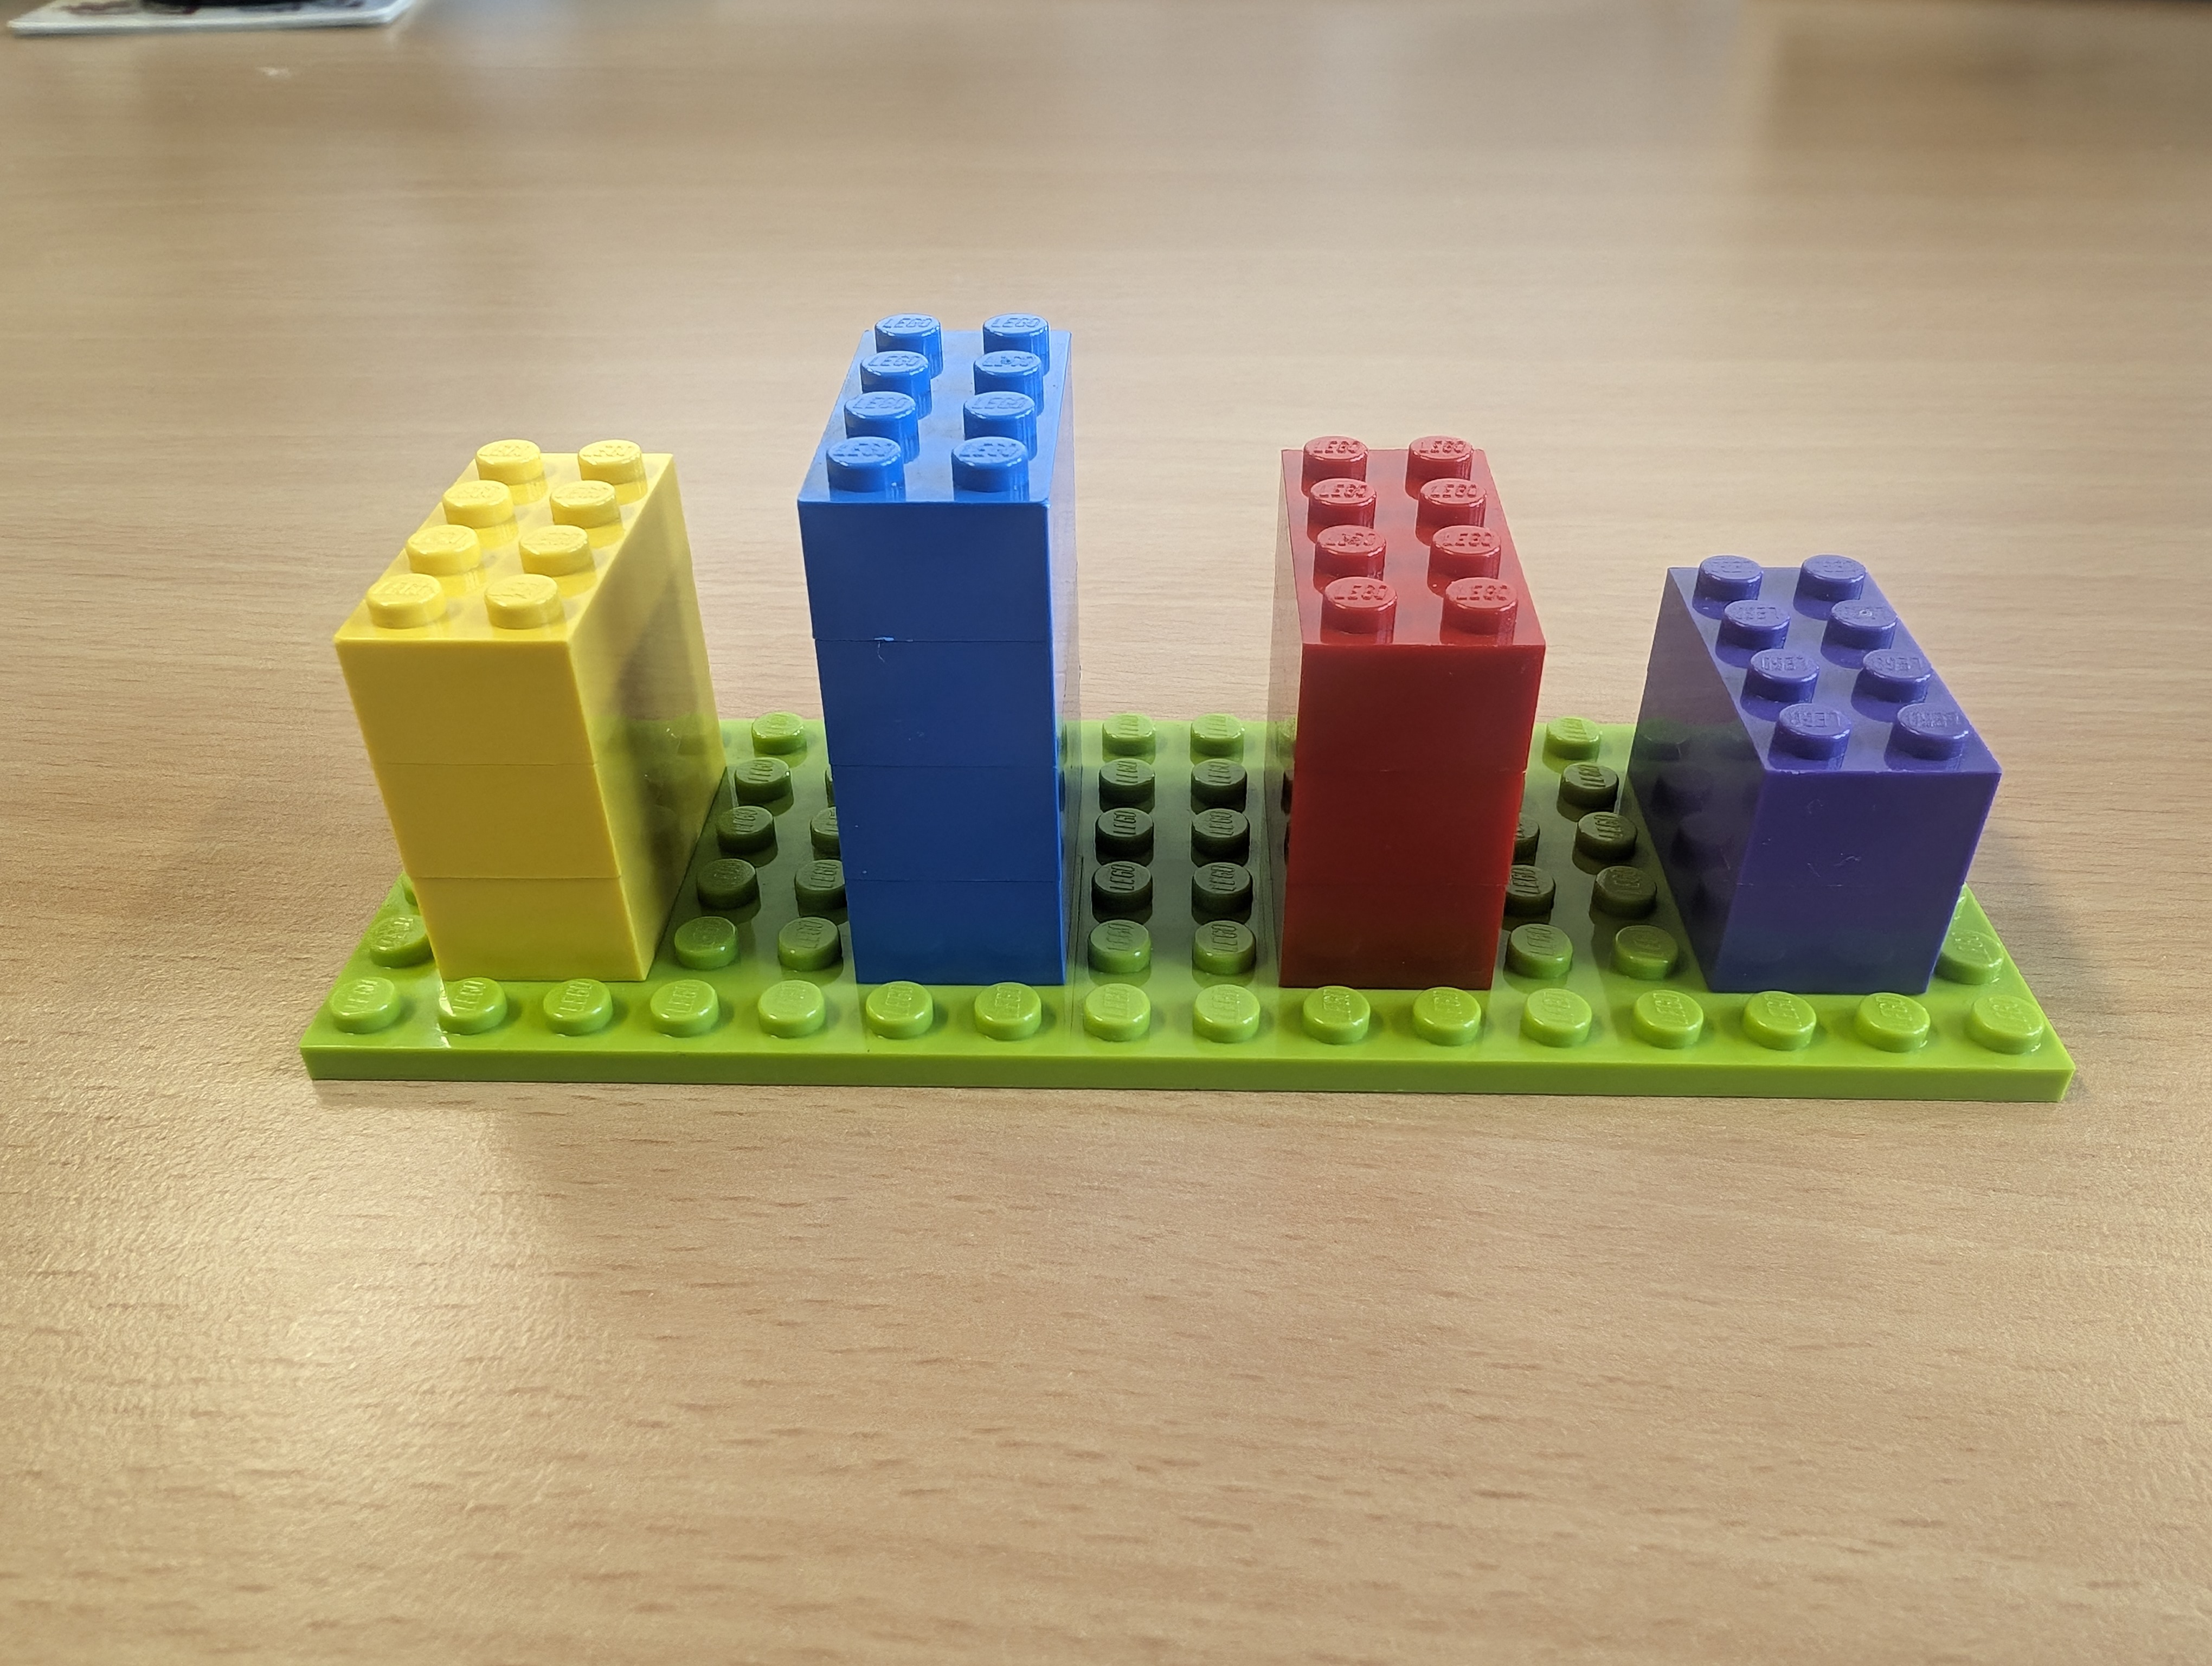
\includegraphics[width=\textwidth]{images/lego-1.jpg}
\caption{Initial state}
\end{subfigure}
\begin{subfigure}[b]{0.20\textwidth}
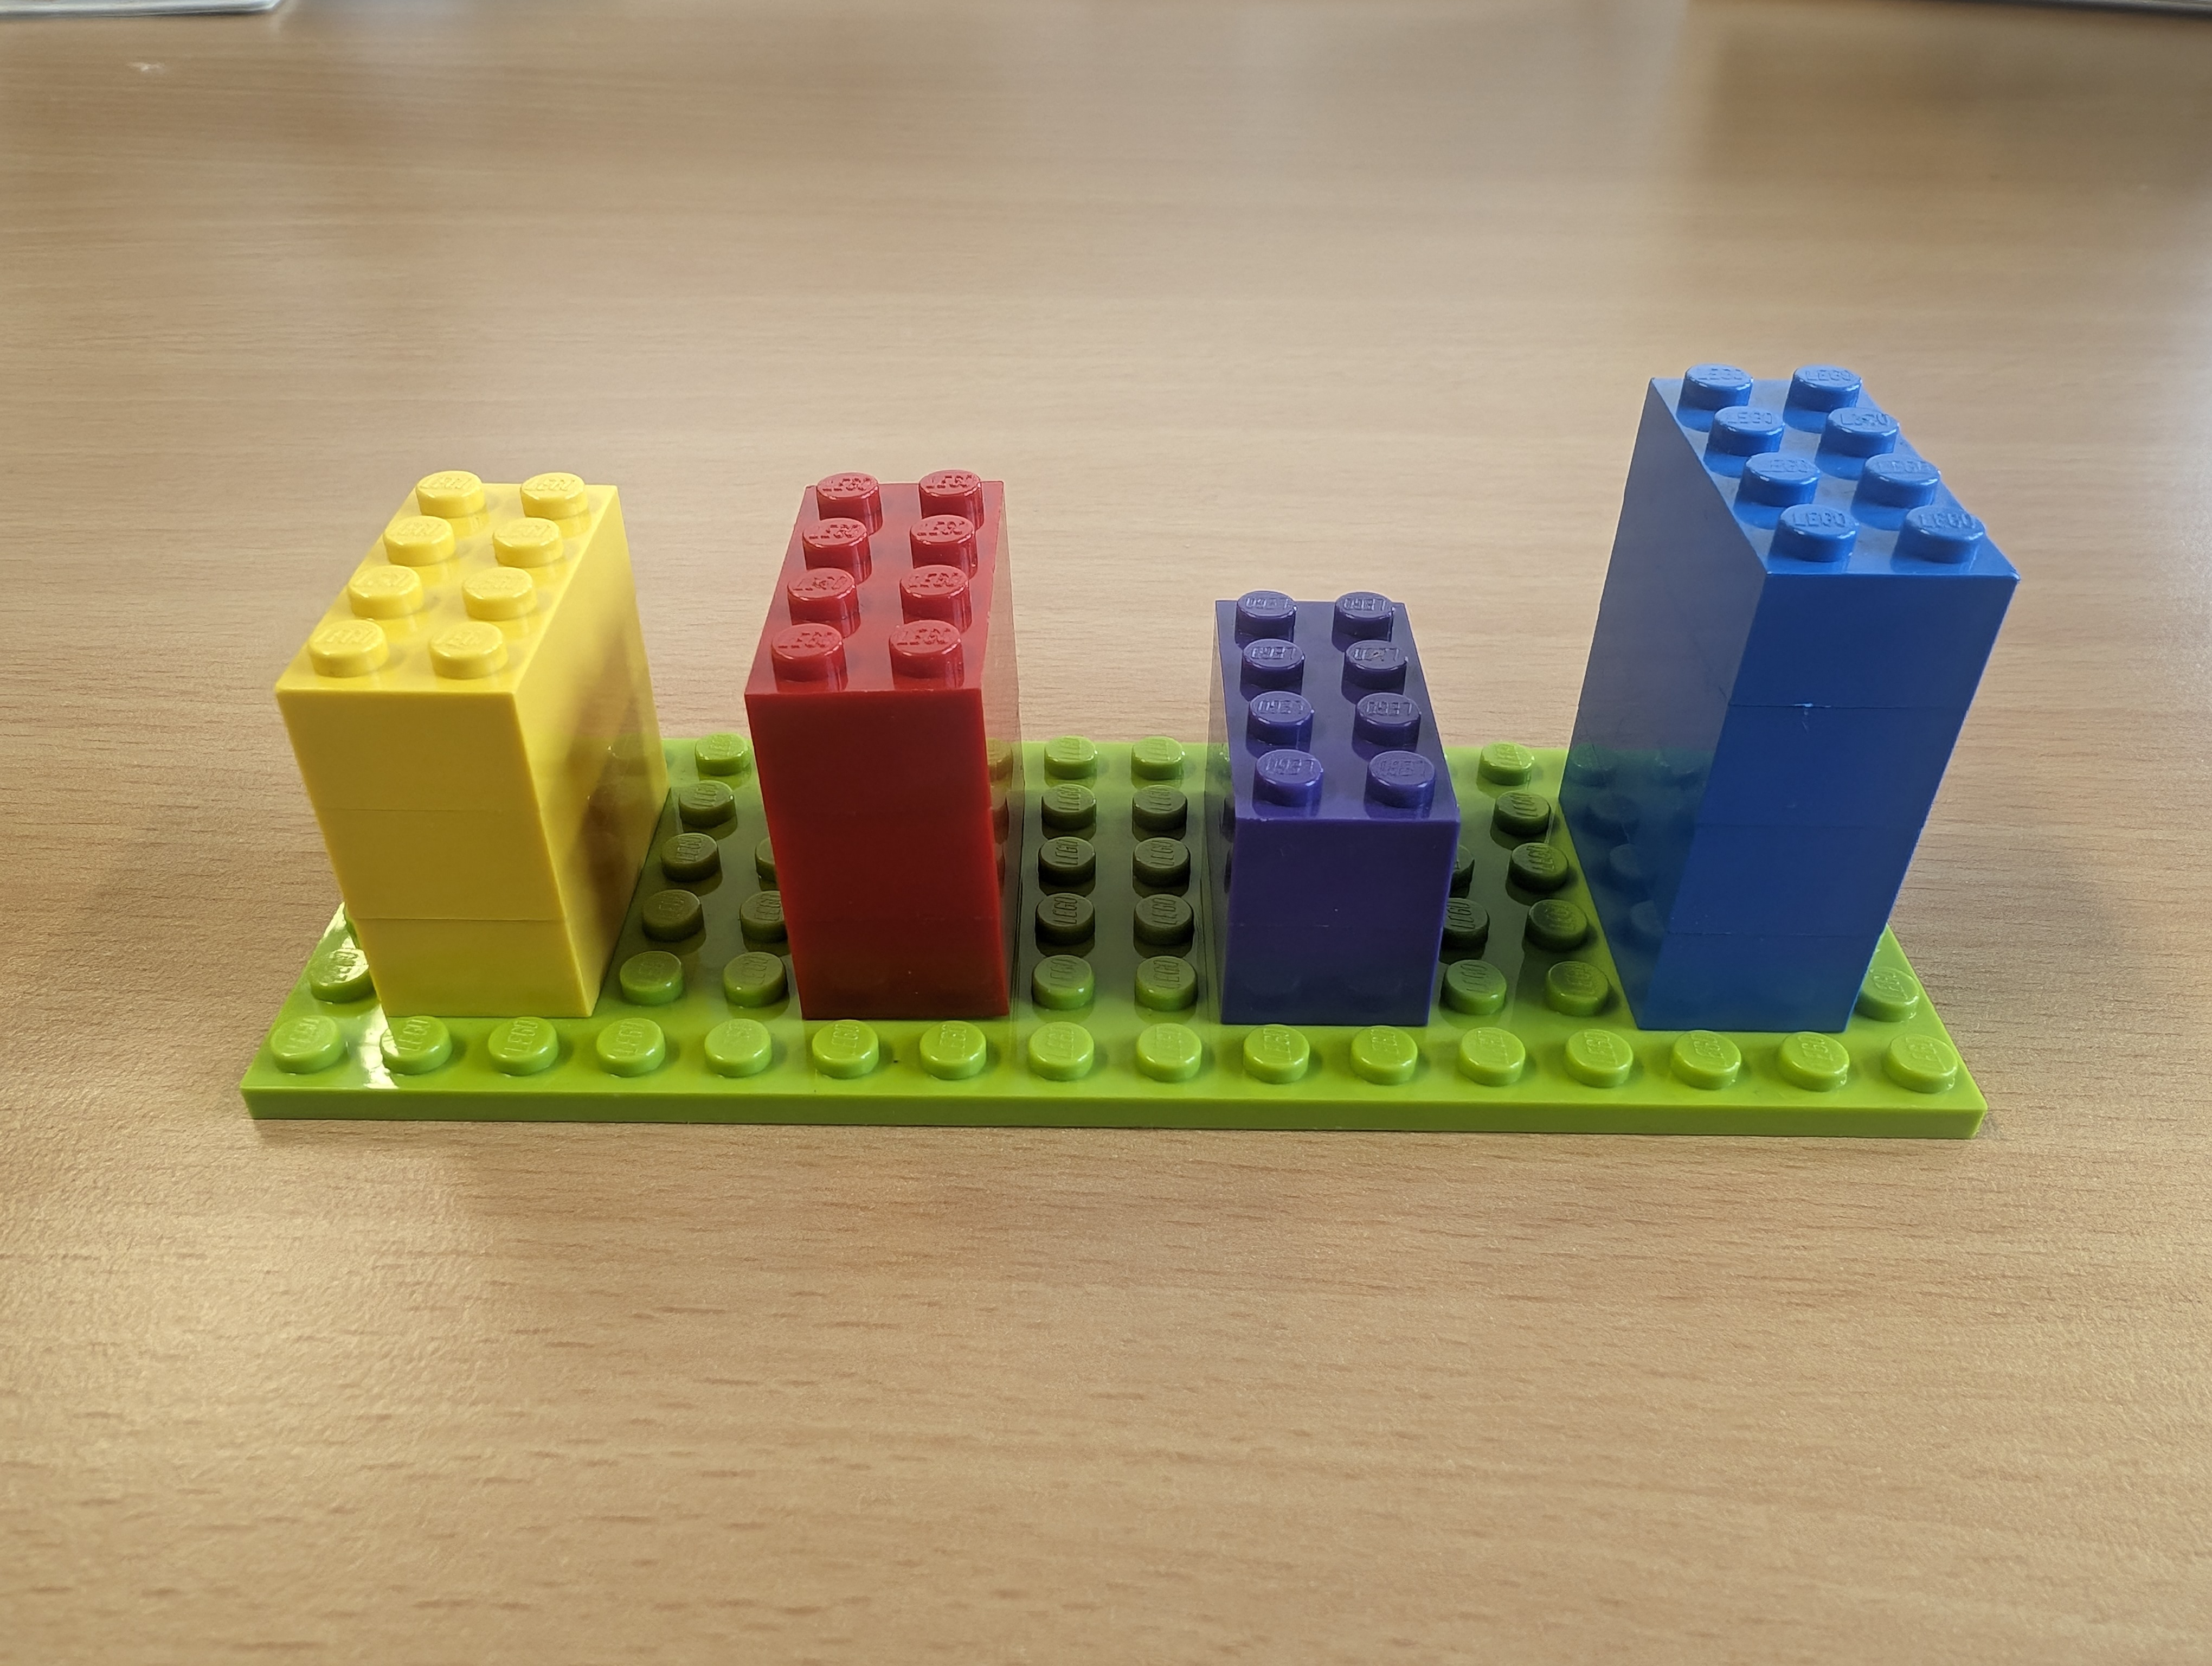
\includegraphics[width=\textwidth]{images/lego-2.jpg}
\caption{First pass}
\end{subfigure}
\begin{subfigure}[b]{0.20\textwidth}
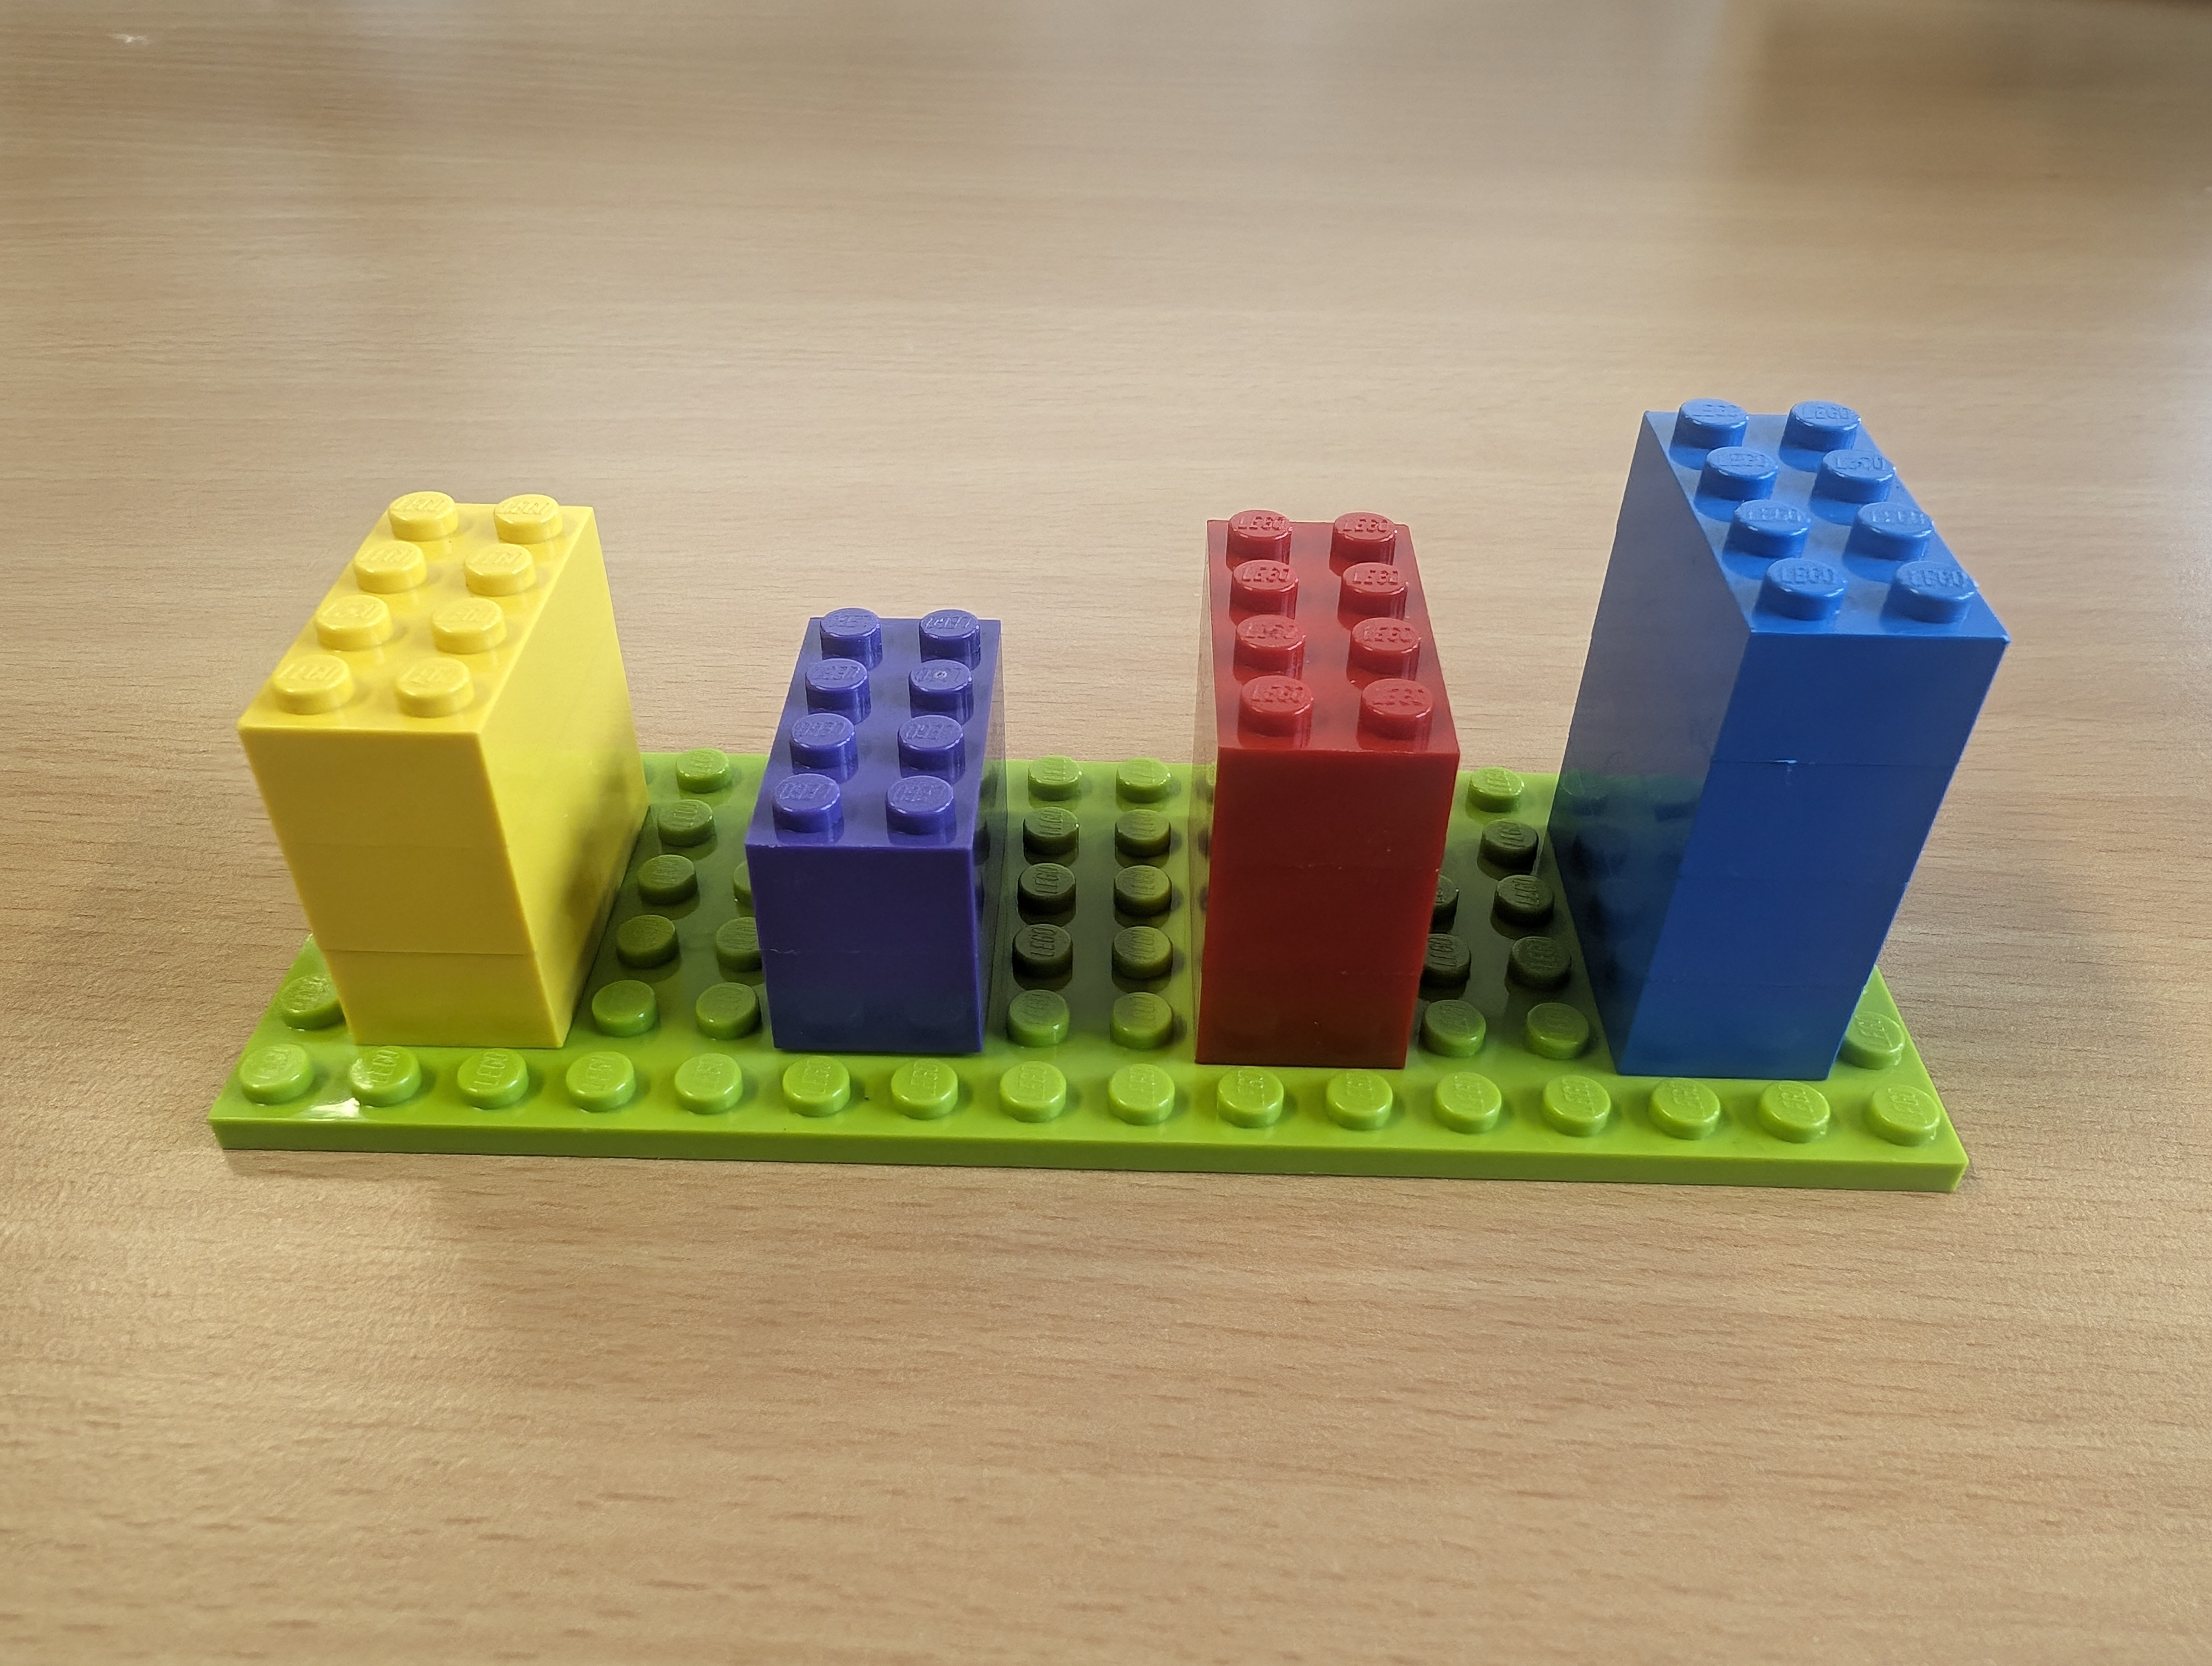
\includegraphics[width=\textwidth]{images/lego-3.jpg}
\caption{Second pass}
\end{subfigure}
\begin{subfigure}[b]{0.20\textwidth}
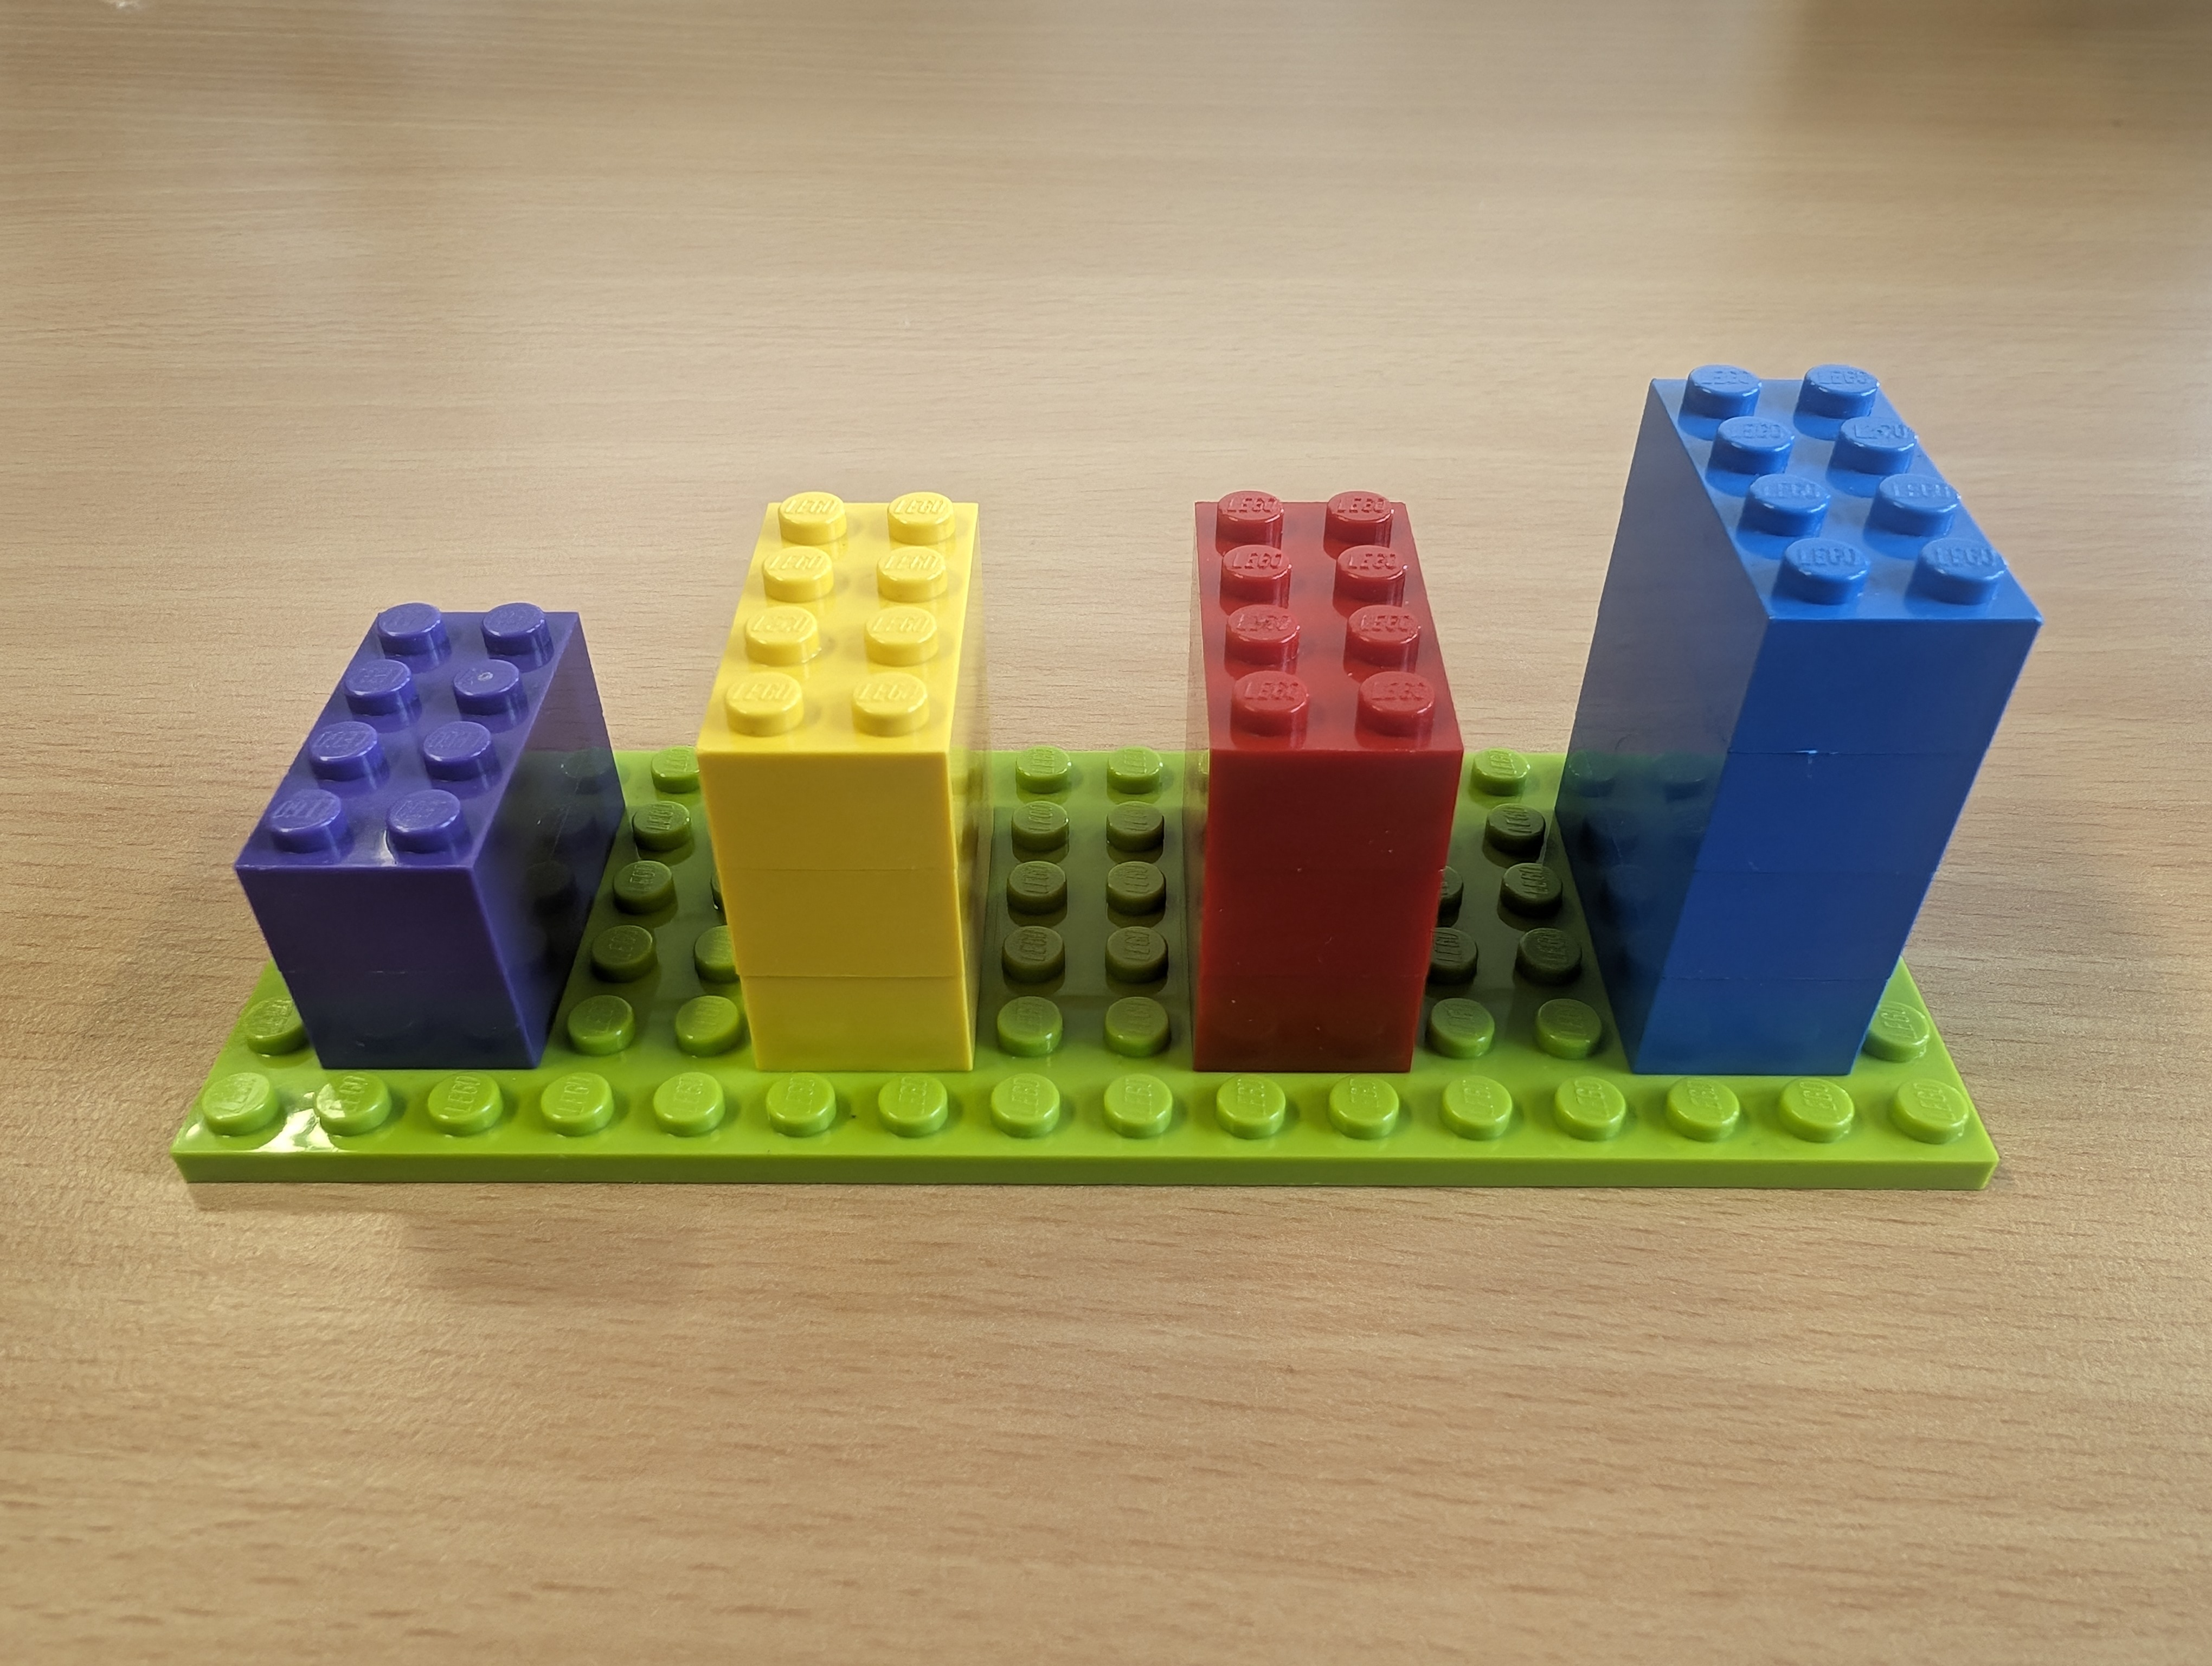
\includegraphics[width=\textwidth]{images/lego-4.jpg}
\caption{End state}
\end{subfigure}
\caption{Multiple toy bricks with different heights to visualize sorting algorithms.}
\label{fig:lego}
\end{figure}

As part of the ''Coding Culture Oberberg'' research project, a workshop was held with a focus on sorting algorithms. One of the goals was to teach the bubble sort algorithm. However, before this was presented in code-based form, it was visualized using toy bricks, which are shown in figure \ref{fig:lego}\footnote{A visual demonstration can be seen at \url{https://th-koeln.sciebo.de/s/l3q4BJ5xdoyTI9T}}. First, participants were able to try out different sorting concepts by using toy bricks of different heights. For this purpose, the procedure of the bubble sorting algorithm was then visualized by the workshop holder using the toy bricks. Before this concept was then transferred to a code-based representation, the participants had time to reproduce the procedure with their own toy bricks.

\subsubsection{Related Pattern}
\begin{itemize}
\item Building Materials: To enable participants to for example build algorithms in a paper-based form, building materials like paper or building bricks are required.
\item Prototyping: The reduce in Overhead through the abundance of real code syntax supports the exploration of a topic and can therefore be used to try out ideas in a first prototype.
\end{itemize}

\subsection{Hands On First}

\subsubsection{Context}

As part of a coding workshop, the educators' main goal is to keep participants motivated and engaged. At the same time, participants should get hands-on experience about the learned concepts. When planning the sequence of a workshop, educators consider different established approaches.

\subsubsection{Problem}

The traditional design includes an initial theoretical input, with hands-on practice later on. This workshop design reduces the motivation of the participants, as they have to wait to work independently. This can lead to a decrease in the participant's commitment to the workshop.

\subsubsection{Forces}

\begin{itemize}
\item {\textbf{Target Group}}: Especially with a younger target group, it is important to pick them up early, as they lose motivation more quickly due to a shorter attention span. The reduced motivation further exacerbates their already limited attention span, compounding the challenge of maintaining active participation.
\item {\textbf{Motivation}}: The motivation of the participants is crucial for the success and the execution of the workshop.
\item {\textbf{Early Impression}}: During a workshop, the focus is on the initial introductory part as it is largely responsible for the success and atmosphere within the workshop and therefore a priority.
\item {\textbf{Complexity}}: When teaching complex topics, some prior knowledge may be required.
\item {\textbf{Redundancies}}: Depending on the prior knowledge of the participants, a frontal input can contain redundancies and thus reduce the motivation of some participants to a greater extent.
\item {\textbf{Learning Preferences}}: Different participants have different preferences in terms of how knowledge should be conveyed. Although those preferences don't impact the actual learning process, they can influence participants' motivation.
\item {\textbf{Interaction}}: Frontal input only allows very limited interaction for the participants.
\end{itemize}

\subsubsection{Solution}
\emph{Introduce an initial practical part as the starting point of the workshop}
\\
Instead of a frontal input as an introduction, the workshop should start with a practical part. This practical phase focuses on the interactive examination of the given topic. The teacher should allow the interactive exploration of the topic and act as support for learners if problems or barriers occur.
This approach is also supported by the learning orientation ''constructivism'', which describes learning as the process of learners actively constructing knowledge. The learner is an active participant in the process and requires engagement.

As this solution describes an initial hands-on part, the example from the \textit{Code without Code} pattern can be applied here. In the context of learning basic algorithms, participants can freely experiment with the existing building blocks to get a first understanding of a new topic. Afterward, further explanation should be provided by the workshop leader. For this running example, it is important to note that the solution of \textit{Hands-on first} is not only restricted to get hands-on with physical objects but can also allow for an initial exploration in code.

\subsubsection{Consequences}

\paragraph{Benefits}

\begin{itemize}
\item An initial practical part allows the workshop leader to get a \textbf{first impression} of the participants' cognitive level and prior knowledge to adjust the workshop accordingly.
\item Exploring a topic independently supports \textbf{individual learning speeds}.
\item Going hands-on with a topic \textbf{increases} the participant's \textbf{motivation}, especially with a younger target group.
\item For the following parts of the workshop, participants can \textbf{fall back on} their \textbf{practical experience}, which can lead to a sense of achievement and positive emotions.
\item An initial Hands-On part with optional guidance by an educator supports \textbf{experience-based learning}.
\item A practical introduction can be used to convey a new topic, but also to sum up and \textbf{recollect prior knowledge}.
\end{itemize}

\paragraph{Liabilities}

\begin{itemize}
\item \textbf{Depending on the topic and prior knowledge}, a practical introduction might not be possible.
\item Working independently \textbf{requires} some amount of \textbf{prior knowledge}.
\item A practical part at the beginning can set \textbf{false expectations} for the rest of the workshop.
\item Additional \textbf{preparation} from the workshop supervisor is required.
\item Learners might be \textbf{too shy to ask} the workshop leader for support.
\item For some participants, an initial practical part might be \textbf{less fun} and therefore hinder their motivation.
\end{itemize}

\subsubsection{Known Uses}

\begin{figure}[htbp]
\centering
\begin{subfigure}[b]{0.5\textwidth}
\includegraphics[width=\textwidth]{images/hourofcode.png}
\caption{A collection of possible ”Hour of Code” coding activities}
\end{subfigure}
\begin{subfigure}[b]{0.5\textwidth}
\includegraphics[width=\textwidth]{images/hoc-application.png}
\caption{Exemplary Hour of Code task ''Hello World: Transformers One''}
\end{subfigure}
\caption{The application ''Hour of Code'', which consists of smaller individual learning tasks.}
\Description{The picture shows the application Hour of Code, which consists of multiple smaller learning tasks for introductory programming.}
\label{fig:hourofcode}
\end{figure}

%\begin{figure}[!h]
%  \centering
%  \includegraphics[width=0.5\linewidth]{images/hourofcode.png}
%  \caption{A collection of possible ''Hour of Code'' coding activities}
%  \Description{}
%  \label{fig:hourofcode}
%\end{figure}

The ''Hour of Code'' is an international initiative to promote computer science in an educational context. Specifically, it is a concept that provides various activities and learning videos to give learners of all levels an insight into programming within one hour. Hour of Code includes an extensive collection of different learning resources and tasks, which can be used by interested teachers after registering for an event. Thanks to the community-driven approach, this collection is regularly expanded. Hour of Code is already used by over 400 partners and over 20,000 teachers. Figure \ref{fig:hourofcode} shows an exemplary overview of some activities on offer. \footnote{\url{https://code.org/hourofcode}, last accessed February 16, 2024}

The ''Hour of Code'' initiative aligns with the ''hands-on first'' approach by providing learners with interactive activities, tasks and learning videos aimed at demystifying computer programming concepts within a short timeframe. This approach emphasizes active engagement and practical exploration, allowing learners to dive into coding concepts quickly and experiment with real code examples.

\subsubsection{Related Patterns}
\begin{itemize}
\item \textbf{First Steep}: \textit{First Steep} supports the idea of straight jumping into an interesting sounding topic and following your intuition alongside. This idea aligns with the solution of \textit{Hands-on first}, which supports the exploratory introduction into a new topic.

\item \textbf{Prototyping}: Prototyping your ideas, can support the aspect of exploring a new topic. Participants can therefore validate or iterate their ideas.
\item \textbf{Students Decide}: \textit{Students Decide} supports the idea of student leading the topic of a class, based on their interests and expectations. This can also be applied to the structure of a Coding Workshop.
\end{itemize}

\subsection{Teamwork makes the dream work}

\subsubsection{Context}
In coding workshops, there exists a variety of potential teaching formats. The traditional approach to convey knowledge relies on independent application of solutions to provided tasks.

\subsubsection{Problem}
If workshop participants work on tasks individually, they can only draw on their own skill set and thus only consolidate their own strengths and weaknesses. It is not possible to benefit from the knowledge of other participants.

\subsubsection{Forces}
\begin{itemize}
\item \textbf{Motivation:} Encountering frequent dead ends in problem-solving can be demotivating, especially when learners feel they lack the resources or guidance to overcome obstacles efficiently.
\item \textbf{Isolated Learning Experience:} Without opportunities for discussion and collaboration, learners may feel isolated in their learning journey, hindering their ability to explore concepts deeply.
\item \textbf{Limited Discussion Opportunities:} In a traditional workshop setting, the instructor typically serves as the sole point of contact for questions and discussions. This limitation restricts the diversity of perspectives and solutions available to learners.
\item \textbf{Instructor Dependency:} Relying solely on the instructor for guidance creates a hierarchical learning environment that may discourage learners from seeking help, thereby limiting their growth and understanding.
\end{itemize}

\subsubsection{Solution}
\emph{Introduce collaborative approaches in coding workshops.}
\\
Collaborative approaches like Pair Programming and group tasks encourage team members to engage actively, share knowledge, and collectively tackle coding challenges. This process fosters collective learning and mutual support among participants.

Based on the previous running examples, the explained solution can also be applied to a coding workshop for learning basic algorithms. \textit{Teamwork makes the dream work} can be applied at multiple times across the workshop. The first example would be an initial hands-on first part, where participants can freely explore the given topic. When also applying the \textit{Code without Code} solution, multiple participants could try to build algorithms from paper building blocks in groups. They can therefore discuss solutions and possible outcomes. \textit{Teamwork makes the dream work} can also be applied when doing real coding, for example when doing pair programming.

Additionally, it's important to consider the optimal group size when implementing collaborative learning strategies, as well as ensuring an equal distribution of tasks among participants to prevent overburdening certain individuals and underutilizing others. Choosing an appropriate group size ensures effective communication and collaboration among participants. For example, smaller groups may facilitate more active participation and individual engagement, while larger groups can provide diverse perspectives and collective problem-solving abilities. Carefully selecting the group size is a crucial aspect of successfully implementing collaborative approaches in coding workshops. A maximum group size of four participants is recommended.

\subsubsection{Consequences}

\paragraph{Benefits}

\begin{itemize}
\item Collaborative approaches in coding workshops facilitate a more engaging and interactive learning environment, where participants can \textbf{benefit from diverse perspectives} and collective problem-solving, leading to a deeper understanding of coding concepts.
\item By mitigating quick dead ends and providing opportunities for mutual support, collaborative learning fosters a supportive atmosphere that encourages participants to persevere through challenges, leading to increased \textbf{motivation} and confidence.
\item Breaking \textbf{away from isolated learning experiences} allows for more extensive discussions and knowledge exchange among peers, enriching the learning process and promoting deeper understanding of coding principles.
\item Encouraging collaboration \textbf{reduces} the \textbf{dependency on a single instructor}, opening up access to a wider range of learning resources and expertise within the group, thereby enhancing the quality and diversity of learning experiences.
\item Explaining concepts to peers reinforces understanding, making collaborative learning an effective \textbf{method for comprehension}.
\item Collaboration ensures that all members contribute to and benefit from the collective effort, promoting \textbf{equitable skill development}.
\item In addition to technical skills, collaborative learning nurtures essential \textbf{soft skills} like teamwork, communication, and problem-solving.
\item Collaborative learning encourages participants to \textbf{engage on multiple levels}, fostering deeper involvement and understanding. Especially fast learners find value in collaborative tasks, as they provide opportunities for further exploration and contribution after completing given tasks.
\end{itemize}

\paragraph{Liabilities}

\begin{itemize}
\item In collaborative settings, there is a risk of some participants contributing more than others, leading to \textbf{uneven skill development} and a lack of \textbf{fairness} in workload distribution.
\item Participants may \textbf{gravitate towards tasks they are already proficient} in, limiting opportunities for skill development in new areas.
\item The effectiveness of collaborative learning relies heavily on the \textbf{dynamics within the group}. Disruptions or conflicts among team members could hinder the learning process and negatively impact the overall experience.
\item Finding the right balance between providing autonomy for individual learning and offering guidance within a collaborative framework can be challenging, as it requires careful management to ensure that participants receive \textbf{adequate support} while still having the opportunity to \textbf{explore independently}.
\item Collaborative environments may inadvertently lead to \textbf{groupthink}, where participants conform to the dominant ideas within the group, \textbf{limiting critical thinking and creativity}.
\end{itemize}

\subsubsection{Known Uses}

\paragraph{Pair Programming}

\begin{figure}[h]
\centering
\includegraphics[width=0.5\linewidth]{images/pairprogramming.png}
\caption{A visualization of ''Pair Programming''\protect\footnotemark}
\label{fig:pair}
\end{figure}
\footnotetext{\url{https://www.linkedin.com/pulse/when-implement-pair-programming-getinrhythm/}, last accessed September 26, 2024}

Pair programming is a technique where two persons work together at one computer, while developing software. One person takes the role of the driver. The Driver writes the code while the other person, named the navigator, reviews each line of code as it's been written. For the best results, both persons should be in both positions at least once. This collaborative approach fosters continuous feedback, leading to higher code quality and fewer bugs. Pair programming also promotes knowledge sharing and helps team members learn from each other's expertise.

\subsubsection{Related Patterns}
\begin{itemize}
\item \textbf{Community of Learning}: \textit{Community of Learning} supports the idea of learning together in a group, as the individual capacity is limited. This aligns with the solution of \textit{Teamwork makes the dream work}.
\item \textbf{Release of Thought}: While working together as a team, participants are able to talk about their ideas with others. They therefore get a chance to reflect upon their ideas.
\item \textbf{Ice Breaker}: The idea behind \textit{Ice Breaker} is to provide an activity for a group to get them to interact with each other, so there is no awkward moment among new group members.
\item \textbf{Open-Process Learning}: \textit{Open-Process Learning} is about opening your learning process to others. This allows the exchange and discussion of ideas.
\end{itemize}

\subsection{Connect the pieces}

\subsubsection{Context}
In a coding workshop, different contents, which are related to a bigger topic, are taught. Even if these topics belong to a common domain, they are initially treated separately and independently of each other.
This approach aligns with the principle of ''Divide \& Conquer'', breaking down complex subjects into smaller, more manageable units. Furthermore, in consideration of the cognitive load theory, the separate introduction of individual theory leads to a reduction in the cognitive burden on participants.

\subsubsection{Problem}
Participants are unable to detect the relevance of the individual topics in relation to each other and to the common topic. This lowers the motivation of the participants and thus reduces their commitment to the workshop.

\subsubsection{Forces}

\begin{itemize}
\item \textbf{Domain specific knowledge}: Since the taught topics are new to the participants, not everyone has the domain specific knowledge for the common topic.
\item \textbf{Limited attention span}: Participants only have a limited attention span and can therefore not memorize all individual topics.
\item \textbf{Engagement}: Initially seemingly unrelated topics can reduce participant engagement.
\item \textbf{Purpose}: Participants might not see the purpose in learning seemingly unrelated topics.
\item \textbf{Application of knowledge}: It might be hard for participants to apply individual topics in the real world without further context.
\end{itemize}

\subsubsection{Solution}

\emph{Implement a moment in the workshop where all previous topics are connected and put in relation.}
\\
During the workshop, there should be a moment when the topics that have so far been considered independently of each other are placed in relation to each other and to the common theme. It is important that participants can see and understand a coherent picture from the individual topics. At this point, the topics should also be placed in relation to the general domain.
The appropriate time to connect the pieces can either be towards the end or after each individual subtopic that adds to the greater domain.

The presented solution can also be applied to the running example. \textit{Connect the pieces} should act as the highlight of the workshop. Applying this to the topic of learning basic algorithms, a possible outcome can be the linking of previously learned algorithms, which at first may seem to be unrelated to each other. Another possibility is to show how the previous algorithms can act as a foundation for a bigger and more complex algorithm.

\subsubsection{Consequences}

\paragraph{Benefit}

\begin{itemize}
\item Linking multiple topic together leads to a \textbf{deeper understanding}.
\item Recognizing relations between topic and their relevance can increase participants' \textbf{motivation}.
\item Linking previous topic together can be a \textbf{highlight} of the workshop.
\item The linking of topics gives \textbf{more structure} to the workshop.
\item Linking topic together can trigger a \textbf{surprise effect} for the participants.
\item Recognizing relations between topics can motivate participants to \textbf{dive further} into a topic on their own.
\item The separation into different subtopics in the beginning inherently conveys the divide and conquer paradigm, which plays an important role in the realm of computer science.
\end{itemize}

\paragraph{Liabilities}

\begin{itemize}
\item The linking of topics needs to be planned and therefore leads to an \textbf{increased preparation effort}.
\item To recognize all relations between topics, \textbf{every individual topic must be understood} at least to a certain degree.
\item Linking multiple topics and therefore summarize them again, can be seen as a \textbf{redundancy} from the participants which can lower the attention.
\item Not every topic can be \textbf{partitioned} into small logical chunks.
\end{itemize}

\subsubsection{Related Patterns}
\begin{itemize}
\item \textbf{Hidden Connections}: \textit{Hidden Connection} supports the idea of finding hidden connections among topic. The allows for a new perspective on already known topics and therefore aligns with the concept of \textit{Connect the pieces} to paint a bigger picture for workshop participants.
\item \textbf{Larger than Life}: \textit{Larger than life} supports the idea of giving students a big complex topic upfront and slowly work towards that topic. Even though this is contrary to \textit{Connect the Pieces}, a switch in perspective could be used in a coding workshop.
\end{itemize}

\subsection{Take It Home}

\subsubsection{Context}

The pivotal point of coding workshops lies in knowledge dissemination, which involves the effective transfer of information and skills from the facilitator to the participants. Most of these workshops are self-contained, lacking subsequent tasks or assignments as well as follow-up workshops. Upon the conclusion of coding workshops, learners leave the knowledge field that was taught.

\subsubsection{Problem}

Participants face challenges retaining coding concepts post-workshop without reinforcement. This inability to retain knowledge leads to a decline in proficiency and limited application of learned skills. This challenge primarily stems from the absence of regular repetition of the acquired content.

\subsubsection{Forces}

\begin{itemize}
\item{\textbf{Application Challenges}}: Implementing learned skills becomes difficult without consistent practice.
\item{\textbf{Fading Memories}}: Event if participants want to repeat the new skills, details from the workshop might be diminished after some time, hindering the recall of crucial concepts.
\item{\textbf{Diminished Motivation}}: Without tangible reminders or continuous support, participants' enthusiasm wanes for applying newfound knowledge.
\item{\textbf{External Distractions}}: Engagement with other events might distract learners from the acquired knowledge and impact retention.
\item{\textbf{Missing Hardware}}: Not every workshop participant owns appropriate hardware, to apply the newly acquired knowledge at home.
\end{itemize}

\subsubsection{Solution}
\emph{Gift tangible artifacts for enhanced retention}
\\
Deliver a tangible artifact to participants at the workshop's conclusion. This artifact, whether physical or digital, serves as a continuous reminder of key lessons, encouraging individuals to enhance their newly acquired skills. It ideally doubles as a tool to retrace developed solutions. This highlights the importance of its practical relevance beyond mere play. Small objects are particularly effective in this context, because they can be taken anywhere to bring the reminder into different environments.

To further emphasize the artifacts' purpose beyond mere mementos, it is crucial that these items are directly linked to the workshop's core content, providing a tangible means for participants to revisit and practice the learned material. This approach transforms the artifact from a simple keepsake into a functional component of the learning experience, extending its educational impact well beyond the workshop setting.

For applying this solution, it is possible to build up upon the previous running examples. If appropriate for the topic of the workshop, the hands-on building blocks from the \textit{Hands on first} pattern can be gifted to the workshop participants. Sticking to the example of learning basic algorithms, participants could use the building blocks at home to either repeat the topics from the workshop or try to solve new algorithmic problems.

\subsubsection{Consequences}
\paragraph{Benefits}

\begin{itemize}
\item Continuous reminders of key concepts fortify participants' ability to retain coding knowledge post-workshop through \textbf{repetition}. As individuals are reminded of key concepts, they are prompted to repeatedly engage with and review the material.
\item The artifact encourages consistent practice, aiding participants in \textbf{applying} coding skills effectively.
\item Connections fostered through the artifact stimulate interest, prompting deeper exploration and understanding of workshop content to increase \textbf{motivation}.
\item The lasting impression of the memory artifact potentially generates more recommendations and \textbf{follow-up workshops}, as participants can \textbf{share their experience} with others.
\end{itemize}

\paragraph{Liabilities}

\begin{itemize}
\item There's a risk that the artifact's novelty wears off quickly, potentially leading to its rapid \textbf{forgetfulness or displacement} from participants' attention.
\item Participants might become \textbf{overly reliant} on the memory artifact, neglecting other revision methods, impacting their ability to engage in diverse learning approaches effectively.
\item The increased disposal of artifacts, particularly in large quantities, might pose challenges in waste management and negatively affect \textbf{environmental sustainability}.
\item The use of unfitting objects can lead to \textbf{distraction} from the actual content
\item Preparing tangible artefacts for every workshop participant results in \textbf{additional labour and costs} for the workshop leader. This increases with the number of participants.
\end{itemize}

\subsubsection{Known Uses}

\paragraph{Coding Culture}

\begin{figure}[h]
\centering
\begin{subfigure}[b]{0.23\textwidth}
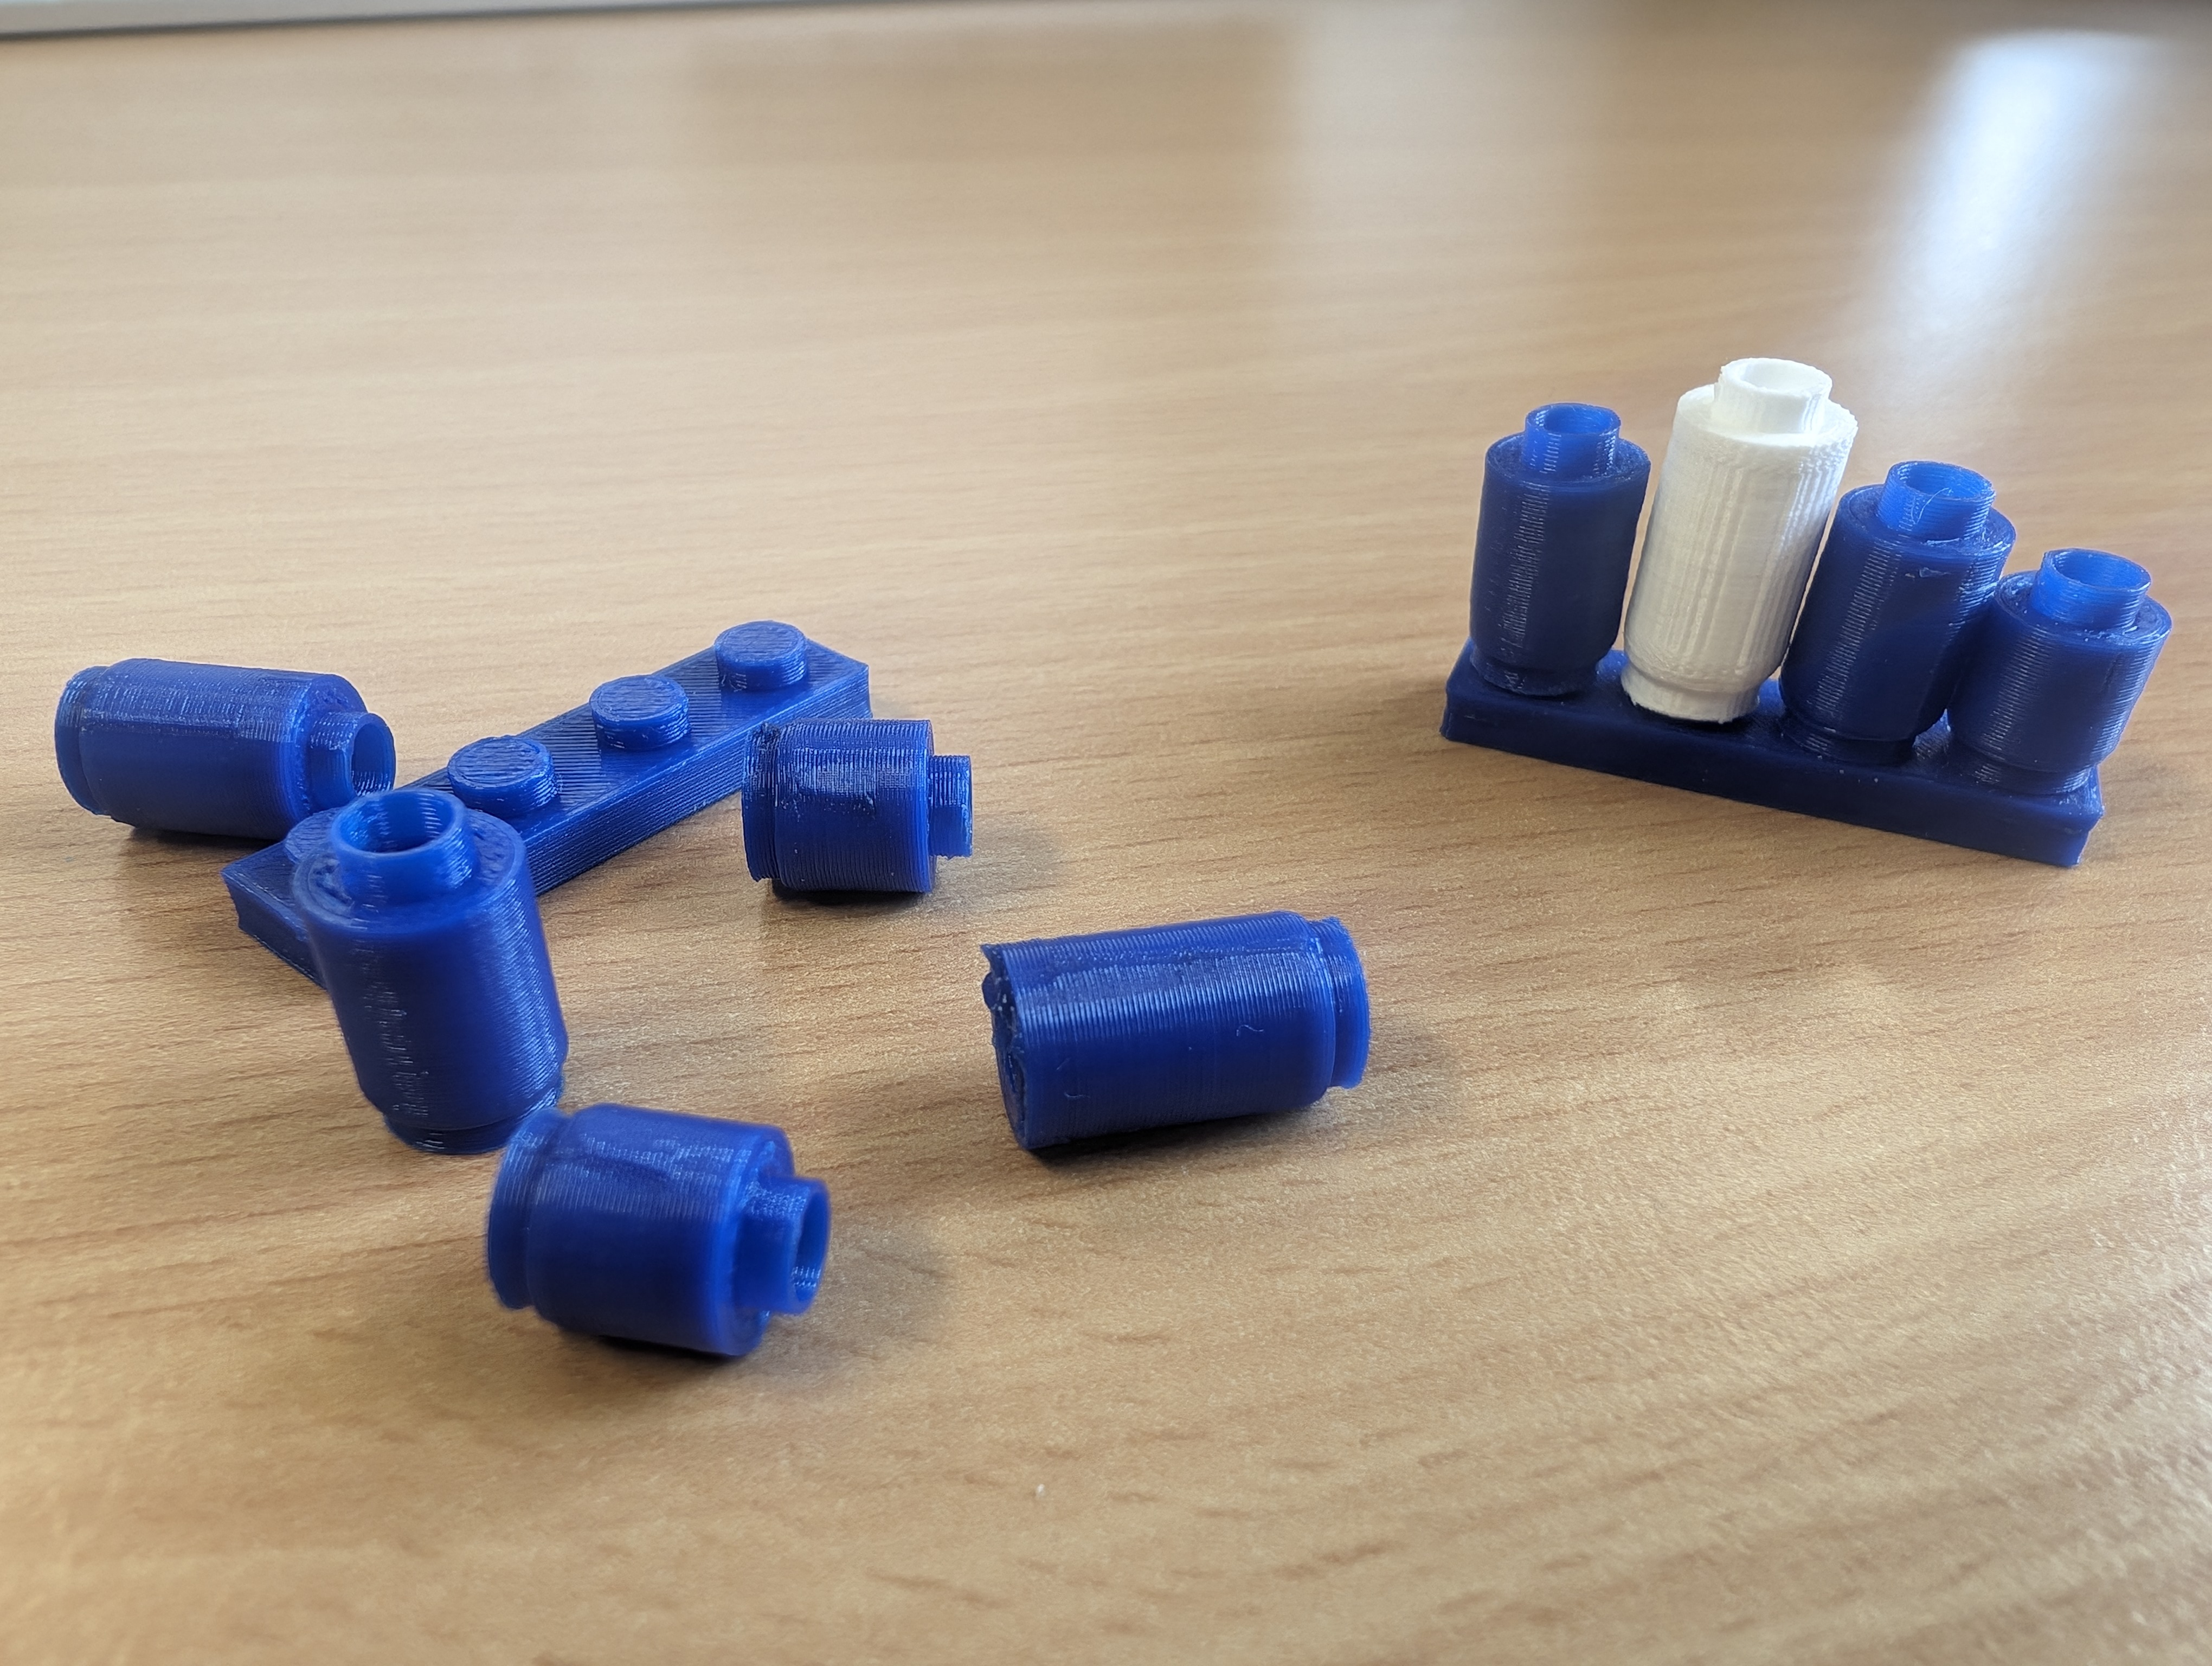
\includegraphics[width=\textwidth]{images/3d-print.jpg}
\caption{3D-printed object}
\end{subfigure}
\begin{subfigure}[b]{0.23\textwidth}
\includegraphics[width=\textwidth]{images/lego.jpg}
\caption{Common toy bricks}
\end{subfigure}
\caption{Comparison of 3D-printed object and bricks used in the workshop}
\label{fig:3d}
\end{figure}

During the ''Coding Culture in Oberberg'' research project, a workshop was conducted for students age 11 to 13. Within this workshop, the Bubble Sort algorithm was taught. At the conclusion of the workshop, each participant received a 3D-printed artifact as a physical object, shown in figure \ref{fig:3d}, representing the approach used to teach the Bubble Sort algorithm. During the workshop, participants sorted towers themselves, a process that can also be carried out using the artifact.

\paragraph{Pattern Coins}

At EuroPLoP 2023, the Iba Lab at Keio University brought coins, as seen in figure \ref{fig:coins}, intended to facilitate the exchange and practice of patterns within a conference context. These coins contain essential information about the patterns they represent.
They serve the purpose of gift-giving as an act and spreading patterns in a community that might benefit from their use. The continuous confrontation with patterns in various contexts as well as the conversations the gift giving sparks leads to retention of their content and greater application.

\begin{figure}[h]
\centering
\includegraphics[width=\linewidth]{images/pattern-coins.jpeg}
\caption{Wooden pattern coins from EuroPLoP 2023}
\Description{}
\label{fig:coins}
\end{figure}

The concept of Pattern Cards serves a similar purpose and is also commonly used within the pattern community.

\subsubsection{Related Patterns}
\begin{itemize}
\item \textbf{Output-Driven Learning}: \textit{Output-Driven Learning} supports the idea of working towards a concrete output at the end of a learning session. This can be applied to where for example concrete buildings blocks are being build and can then be gifted to the participants as part of \textit{Take it home}.
\item \textbf{Embodied Skills}: Continuous practice can help to acquire a desired skill. Giving participants something to take home, enables them to repeat the topic of the workshop or solve open questions.
\end{itemize}

\subsection{Abstract Guided Instruction Through Storytelling}
\begin{figure}[h!]
\centering
\includegraphics[width=0.7\linewidth]{images/agi.png}
\caption{Usage of Abstract Guided Instruction to convey coding concepts through an abstracted representation.}
\Description{The educator has expert understanding or a coding concept. Through Abstract Guided Instruction, a representation of the coding concept can be created and indirectly grasped by the learner.}
\label{fig:agi}
\end{figure}
\subsubsection{Context}
Learners are engaging with programming for the first time and have no prior experience. It is essential to introduce and explain various coding concepts to establish a foundation for programming.

\subsubsection{Problem}
Learning coding concepts without any prior experience poses a significant entry barrier, as it requires a completely new way of thinking \cite{medeiros2018systematic}. The success in programming depends on several predictors such as algorithmic thinking, logical reasoning, and mathematical skills, none of which can be assumed as given.

\subsubsection{Forces}

\begin{itemize}
\item \textbf{Intangible Concepts}: Programming concepts are often abstract and difficult to understand, especially without practical examples and lack familiar references learners can relate to.
\item \textbf{Lack of Familiar References}: Many concepts have little to no connection to already familiar topics, complicating comprehension.
\item \textbf{Wrong Implications}: When learners use familiar topics to grasp concepts without guidance of an educator, they might use inappropriate metaphors that lead to wrong implications.
\item \textbf{Computer Anxiety}: Learners often fear using computers, particularly for programming, and generally fear making mistakes, which leads to hesitant and insecure learning \cite{nolan2016role}.
\item \textbf{Cognitive Load}: The cognitive load is high when many diverse new concepts must be learned simultaneously \cite{van2005cognitive}.
\item \textbf{Concept Integration}: It is challenging to recognize and understand the relationships between different programming concepts.
\item \textbf{Sequential Concepts}: Many programming concepts are sequential and build upon each other, making understanding the basics crucial \cite{lister2009further}. If foundational concepts are not fully grasped, it impedes the learning of more advanced concepts or the connections between them.
\item \textbf{Motivation}: Without early successes, learners often lose motivation quickly \cite{santos2013taxonomy}.
\end{itemize}

\subsubsection{Solution}
\emph{Provide a high level of abstraction with minimal interaction by using metaphors within the framework of storytelling.}
\\
A suitable methodology to introduce programming to learners without prior experience involves using teaching methods that offer a high level of abstraction and require minimal direct interaction of learners. This approach allows learners to gradually familiarize themselves with new concepts without becoming overwhelmed. A central role of this approach is the use of Storytelling, which is defined as ''Augment[ing] the transfer of knowledge through a narrative method that uses rhetorical devices to create tension in order to present a fact-heavy topic in the form of a story'' \cite{10.1145/3628034.3628056}. This method can help to link various concepts and present them in an understandable and relatable context. Appropriate metaphors should be used to make abstract programming concepts more tangible. Well-chosen metaphors help avoid misunderstandings and explain complex ideas in a way that is accessible and understandable for beginners. Combining these approaches facilitates the entry into programming and lowers the learning barrier.

\subsubsection{Consequences}

\paragraph{Benefits}

\begin{itemize}
\item The use of storytelling and appropriate metaphors creates a \textbf{connection to familiar concepts}, improving understanding \cite{baldasaro2014storytelling}.
\item Stories are \textbf{easier to remember}, helping learners to better retain concepts \cite{baldasaro2014storytelling}.
\item A methodology with high abstraction and minimal direct interaction requires \textbf{detailed guidance}, leading to quicker successes for beginners.
\item The \textbf{entry barrier} is very low due to the high level of abstraction and resultant accessibility, making it easier for learners to engage with new concepts.
\item This methodology and extensive guidance minimize the room for errors, boosting learners' \textbf{confidence} and \textbf{reducing fear of failure}.
\item Through storytelling, learners can identify with the narrative, which increases \textbf{ learning motivation}.
\end{itemize}

\paragraph{Liabilities}

\begin{itemize}
\item High abstraction and extensive guidance create a very \textbf{restricted framework} with limited flexibility and exploration opportunities, which leads to a linear experience for learners that might be harmful to their natural curiosity.
\item The \textbf{abstract context} can quickly become unsuitable as learners progress and the methodological framework no longer meets their needs.
\item The \textbf{distance from code} due to high abstraction can make the transition from metaphors to text-based code with syntax challenging.
\item With sequential concepts, a frequent \textbf{change of metaphors} may be necessary, complicating understanding and maintaining continuity in the learning process. This process also includes the challenge of creating fitting metaphors for educators.
\end{itemize}

\subsubsection{Known Uses}

\paragraph{Osmo Coding Awbie}
\label{subsub:osmo}

''Osmo Coding Awbie'' is an interactive game designed for children, using physical blocks that interact with an iPad to teach basic coding concepts. Players arrange these tangible blocks in front of the iPad to create sequences of commands that guide Awbie, a playful character, through various adventures in a colorful virtual world.

\begin{figure}[h!]
\centering
\begin{minipage}{0.4\linewidth}
\centering
\includegraphics[width=\linewidth]{images/Awbie.jpg}
\end{minipage}
\hspace{0.05\textwidth}
\begin{minipage}{0.4\linewidth}
\centering
\includegraphics[width=\linewidth]{images/Awbie2.jpg}
\end{minipage}
\captionof{figure}{Coding Awbie App selection screen and level gameplay with use of tangible coding blocks}
\Description{Coding Awbie App level selection screen and level with code blocks to go through the story}
\label{fig:awbie}
\end{figure}

The storytelling revolves around Awbie's journey, filled with challenges and rewards, engaging children through a narrative that makes learning enjoyable. The adventure and treasure hunt theme serves as a metaphor for coding, illustrating concepts such as sequencing and logic in a playful context. The app is shown in figure~\ref{fig:awbie}

\paragraph{How to Code a Sandcastle}

''How to Code a Sandcastle'' is a children's book by Josh Funk that introduces young readers to programming concepts through a delightful story. The book follows Pearl and her robot friend Pascal as they try to build the perfect sandcastle on the beach.

\begin{figure}[h!]
\raggedright
\begin{minipage}[t]{0.31\linewidth}
\centering
\includegraphics[width=\linewidth]{images/sandcastle1.jpg}
\end{minipage}
\begin{minipage}[t]{0.6\linewidth}
\centering
\includegraphics[width=\linewidth]{images/sandcastle2.jpg}
\end{minipage}
\caption{Book cover and inside view}
\Description{Book cover and book content of ''How to Code a Sandcastle''}
\label{fig:sandcastle}
\end{figure}

The book abstracts coding by breaking down the process of building a sandcastle into simple, step-by-step instructions that mirror coding logic. Through its engaging narrative, it explains complex ideas in an accessible way. The story of Pearl and Pascal captures the readers' imagination, making the learning process fun and relatable. The metaphor of constructing a sandcastle effectively conveys the principles of programming, such as planning, sequencing, and debugging, with Pascal the robot representing a computer following coded commands. The book cover and an inside view of the book is shown in figure~\ref{fig:sandcastle}.

\paragraph{Adventures in Coding}

''Hello Ruby: Adventures in Coding'' by Linda Liukas is a book that introduces children to the world of coding through the adventures of Ruby, a curious and imaginative girl. The book combines storytelling with interactive activities to teach foundational programming concepts.

\begin{figure}[h!]
\centering
\begin{minipage}[t]{0.48\linewidth}
\centering
\includegraphics[width=\linewidth]{images/ruby2.jpg}
\end{minipage}
\hspace{0.02\linewidth}
\begin{minipage}[t]{0.48\linewidth}
\centering
\includegraphics[width=\linewidth]{images/ruby3.jpg}
\end{minipage}
\caption{Inside view of the book}
\label{ref:ruby}
\Description{Book Content}
\end{figure}

''Hello Ruby'' uses narrative and visual abstraction to convey coding principles. Ruby's adventures in a whimsical, illustrated world make abstract programming concepts tangible and relatable for young readers. The storytelling is rich and imaginative, capturing children's interest and making the learning process enjoyable. Two examples of storytelling are shown in figure~\ref{ref:ruby}. Each adventure Ruby undertakes serves as a metaphor for various coding concepts. For instance, problem-solving quests and treasure hunts illustrate debugging and algorithmic thinking, allowing children to learn coding in a playful and engaging manner.

\subsection{Block-Based Programming}

\begin{figure}[h!]
\centering
\includegraphics[width=0.7\linewidth]{images/bbp.png}
\caption{Usage of Block-Based Programming to convey code through an abstracted representation as blocks instead of text.}
\Description{Usage of Block-Based Programming to convey code through an abstracted representation as blocks instead of text.}
\label{fig:bbp}
\end{figure}

\subsubsection{Context}
Learners understand the basic concepts behind programming and algorithmic thinking at a high level of abstraction. They want to expand their knowledge and learn how to write syntactically correct code in order to create a working program.

\subsubsection{Problem}
There is a considerable discrepancy between understanding algorithmic processes and the ability to code from scratch. This discrepancy can be described as a difference in the levels of abstraction. Algorithmic thinking requires the learner to think about abstract concepts at a high level because its goal is to build a repeatable process. Writing text-based code with syntax requires the learner not only to apply algorithmic thinking (a new way of thinking for them), but also to translate it into syntax with which they may not be entirely familiar. These two points in the process of learning to code leave open a gap that has not been fully organized. There are no steps between these two points that help visualize the structure of the code or resemble syntax at a level of low abstraction.
Writing code can be seen as a process that provides low- to medium-interaction, using common editors and syntax. This prevents learners from experimenting with the code and feeling free to change things and explore different solutions.

\subsubsection{Forces}

\begin{itemize}
\item \textbf{Cognitive Load}: Linking existing knowledge to new information while aquiring new knowledge can lead to a high cognitive load \cite{van2005cognitive}.
\item \textbf{Barrier to entry}: The barrier to entry can be high for some learners because they have never worked with code or anything like it before.
\item \textbf{Motivation}: Learners' motivation is influenced by the experience they have while learning. Providing an experience that does not meet learners' needs for competence, autonomy, and relatedness can lead to a decrease in motivation~\cite{Ryan2000}.
\item \textbf{Situational interest}: When a learning task has personal relevance, novelty, activity level, and comprehensibility situational interest can be elicited, which is thought to precede and facilitate individual interest.
\item \textbf{Prior Knowledge}: The learner's prior knowledge plays an important role in learning to code. Additionally, the degree to which that knowledge is embedded in the person's mental model can affect their learning experience.
\item \textbf{Self-perception of competencies}: Abstract prior knowledge of programming, especially when concepts are applied to everyday situations, can hinder learners' confidence in their ability to actually write code \cite{CMM08}.
\item \textbf{Fear to use computers}: Learners may experience the negative emotion of anxiety associated with using computers, which can interfere with the learning experience \cite{nolan2016role}.
\item \textbf{Overwhelm}: Text-based programming using syntax can seem complicated and lead to feelings of frustration~\cite{Hu2021} and overwhelm.
\end{itemize}

\subsubsection{Solution}
\emph{Provide high-interaction, low-abstraction learning solutions using Block-Based Programming.}
\\
High-interaction, low-abstraction learning solutions provide something that enables high-frequency interactivity while remaining at a low level of abstraction.
This structure can be created using Block-Based Programming, optionally combined with tangible objects such as microcontrollers.
Block-Based Programming packages coding logic into individual blocks that can be assembled and nested using drag-and-drop in an editor. Using this type of programming language allows learners to create working programs without writing ''real'' code. This provides a low level of abstraction from code that uses typical syntax.
One or more blocks represent a programming concept. The arrangement of blocks is based on the interrelationships of different concepts. For example, there might be a block to set a variable, or a block to ''code'' a loop. These visualizations are designed to represent concepts intuitively. For example, a loop has a shape that allows other blocks to fit in between it (see figure~\ref{fig:block_based_example}), and shows that those other blocks are contained within that loop.

\begin{figure}[h!]
\centering
\begin{minipage}[t]{0.35\linewidth}
\centering
\includegraphics[width=\linewidth]{Figures/Block-based-Example.png}
\caption{MakeCode Editor}
\end{minipage}
\begin{minipage}[t]{0.6\linewidth}
\centering
\centering
\includegraphics[width=\linewidth]{Figures/littlebits_screenshot.png}
\caption{LittleBits Editor}
\end{minipage}
\caption{A screenshot showing how blocks are constructed in a block-based editor to see if a block can contain another block and how they fit together.}
\Description{A screenshot showing how blocks are constructed in a block-based editor to see if a block can contain another block and how they fit together.}
\label{fig:block_based_example}
\end{figure}

The ability to drag and drop code blocks allows learners to interact with the code, such as exploring different ways to solve problems with a few drags and drops. Adding a tangible object to the mix gives learners additional feedback and a tangible representation of their solutions.
Some Block-Based Programming editors offer to switch between the block-based view and the actual syntax of a particular programming language (e.g., Python), sometimes displaying both versions simultaneously. This reduces the gap between abstract concept and actual code further.

\subsubsection{Consequences}

\subsubsection*{Benefits}
\begin{itemize}
\item \textbf{Computer anxiety} can be reduced through regular use with frequent positive experiences \cite{nolan2016role}.
\item Learner motivation through \textbf{relatable application}, \textbf{autonomy} while exploring and \textbf{high interactivity} is increased.
\item Learners \textbf{gain confidence in their competence} to use programming languages by using Block-Based Programming that resembles text-based code with syntax.
\item Block-Based Programming \textbf{reduces the gap} between prior knowledge and text-based code with syntax. Allowing learners to switch between block-based and actual code helps them build mental models, which reduces the gap between abstract knowledge and text-based code with syntax further.
\item The interrelationships and nesting of different coding concepts, such as loops within loops, can be \textbf{represented in detail} and on a \textbf{low abstraction level}.
\item \textbf{Code visualization} and \textbf{pre-defined blocks} help avoid mistakes like typos. It also rewards knowing important keywords like ''loop'' by providing options on how to use them.
\end{itemize}

\paragraph{Liabilities}
\begin{itemize}
\item Block-Based Programming provides a \textbf{framework} that could be considered \textbf{limiting} by learners.
\item Block-Based Programming is \textbf{limited in the concepts} that can be represented, since it is mainly usable for the representation of imperative programming.
\item Despite the reduced gap, the \textbf{transition to text-based code with syntax} can still be challenging for learners and add \textbf{additional complexity}.
\item Using abstract concepts with metaphors can lead to under-challenge and trigger negative learning emotions such as \textbf{boredom or frustration}.
\end{itemize}

\subsubsection{Known Uses}
In the following, known uses have been divided into two main topics, separating Block-Based Programming editors from the tangible objects that can be controlled by those editors.

\paragraph{Editors: MakeCode}

\begin{figure}[h!]
\centering
\includegraphics[width=\linewidth]{Figures/Make_Code_Screenshot.pdf}
\caption{Screenshot of the MakeCode editor for Calliope with a code for a counter from one to ten.}
\Description{Screenshot of the MakeCode editor for Calliope with a code for a counter from one to ten.}
\label{fig:make_code}
\end{figure}

\begin{figure}[h!]
\centering
\includegraphics[width=\linewidth]{Figures/MicroBit_cropped.jpg}
\caption{Image of the micro:bit with the Maqueen\protect\footnotemark extension built into a small robot that can move in all directions and provides sensors as a distance sensor (two ''eyes'' in front).}
\Description{ToDo}
\label{fig:calliope_mini}
\end{figure}
\footnotetext{\url{https://wiki.dfrobot.com/micro_Maqueen_for_micro_bit_SKU_ROB0148-EN}~(last accessed: May 31, 2024)}

MakeCode\footnote{\url{https://www.microsoft.com/de-de/makecode}~(last accessed: May 31, 2024)} is a Block-Based Programming editor. It contains an area that displays the available blocks, organized into categories that are color-coded. For example, a category for loops (shown in green in figure~\ref{fig:make_code}) contains several loop variants that can be added to the programming area on the right by clicking on them. The blocks on the right can be moved around using drag-and-drop and manipulated using keyboard shortcuts. As shown in the top center of figure~\ref{fig:make_code}, MakeCode allows the user to view the code version of the blocks in programming languages (Python and JavaScript). It allows a side-by-side view or a complete switch between views. The code can also be edited and programs can also be written completely in code.

When using MakeCode with supported devices, such as the Calliope mini, it displays the microcontroller on the left side and simulates the code as much as possible on the screen.

\paragraph{Tangible Objects: Calliope mini, micro:bit, LittleBits}

There are several tangible objects that are compatible with Block-Based Programming editors such as MakeCode. The Calliope mini\footnote{\url{https://calliope.cc/}~(last accessed: May 31, 2024)} and micro:bit\footnote{\url{https://microbit.org/}~(last accessed: May 31, 2024)} are similar microcontrollers that provide a set of built-in sensors that can be controlled through programming. There are also expansion kits that include additional sensors, motors, etc. Figure~\ref{fig:calliope_mini} shows an expansion kit of micro:bit with different servo motors and a distance sensor. Both microcontrollers are easy to set up and use with a Block-Based Programming editor. When using expansion kits, libraries are available that provide blocks that can be used for programming. For example, a kit for building a robot provides blocks for setting the speed of a motor.

LittleBits\footnote{\url{https://littlebits.com/welcome}~(last accessed: May 31, 2024)\label{littlebitsfootnote}} are color-coded modular electronic bits that snap together easily with magnets. It is possible to build a variety of working things by snapping the bits together. Figure~\ref{fig:little_bits_example} shows an example project with wiring diagram to illustrate how the bits are used together. The things learners build with littleBits can also be programmed using Block-Based Programming editors.

\begin{figure}[h!]
\centering
\includegraphics[width=\linewidth]{Figures/LittleBits_Example.pdf}
\caption{Pictures of a sample project ''Tug of War'' with the build project on the left side and the wiring diagram on the right side. The images were sourced from the project instructions provided by LittleBits.\footref{littlebitsfootnote}}
\Description{Pictures of a sample project ''Tug of War'' with the build project on the left side and the wiring diagram on the right side. The images were sourced from the project instructions provided by LittleBits.}
\label{fig:little_bits_example}
\end{figure}
\footnotetext{\url{https://classroom.littlebits.com/lessons/invention-4-tug-of-war}~(last accessed: January 24, 2025)}

\subsection{Self-contained kit}
\begin{figure}[h!]
\centering
\includegraphics[width=0.7\linewidth]{Figures/sck.png}
\caption{Components of Self Contained Kits that can be used either by learners directly or through educators.}
\Description{Components of Self Contained Kits that can be used either by learners directly or through educators.}
\label{fig:sck}
\end{figure}
\subsubsection{Context}

Learners, particularly beginners, aim to learn programming using games or kits. This learning takes place either at home in a playful and spontaneous setting or in learning environments such as schools, with educators preparing materials for lessons. Both settings may have limited access to additional resources.

\subsubsection{Problem}

For coding kits or games to be fully functional, additional crafting materials, electronic parts, and connectors are required. This leads to learners not being able to use the materials or incurring additional acquisition effort.

\subsubsection{Forces}

\begin{itemize}
\item \textbf{Motivation}: If the need to purchase additional parts is not known in advance, it quickly decreases motivation. In particular in spontaneous use, the desire to experiment is quickly dampened, reducing the likelihood that the kit will be used again.
\item \textbf{Acquisition Difficulties}: It can be unclear where the required materials can be sourced. Supply shortages can also prevent the timely acquisition of necessary parts or cause prolonged unavailability.
\item \textbf{Financial Resources}: Financial assessment is challenging if the kit is not usable on its own. Individuals with limited financial means or in regions with difficult delivery conditions may not have access to the required additional parts, significantly restricting accessibility.
\item \textbf{Project-Dependent Additional Parts}: Different projects may require different additional parts, increasing the complexity and effort for learners and educators.
\item \textbf{Preparation Time for Educators}: Educators often have limited time to prepare lesson materials. If kits require additional parts or extensive preparation, it increases the workload and reduces the time available for other teaching activities.
\end{itemize}

\subsubsection{Solution}

\emph{A kit should be used that contains all necessary components.}
\\
Self-containment encompasses both hardware and software. On the hardware side, the kit should include all necessary physical components required for the projects, such as various sensors and actuators, connection materials like cables, connectors, and breadboards, as well as microcontrollers or minicomputers to control the hardware.

On the software side, the components should be easily accessible and usable. This includes pre-installed or easily installable software libraries and frameworks needed for the projects, well-documented example codes to serve as starting points for own projects, comprehensive documentation covering all aspects of using the kit from setup to troubleshooting, and step-by-step instructions and tutorials to support the learning process and ease the entry.

In addition, manuals, project ideas, instructions, and other additional materials should be included in the kit.

\subsubsection{Consequences}

\paragraph{Benefits}

\begin{itemize}
\item Learners can start programming immediately without waiting for additional parts.
\item The ability to start right away increases the motivation and interest of learners and educators.
\item Since all necessary components are already included, planning and executing projects becomes simpler and more straightforward for both learners and educators.
\item A comprehensive kit offers a coherent and integrated learning experience specifically tailored for beginners.
\item Purchasing a complete kit provides upfront knowledge of costs, facilitating financial planning.
\item Educators can save preparation time because all necessary materials are already included, allowing them to focus more on teaching and less on material acquisition and preparation.
\item All-in-one kits save \textbf{sourcing effort} and provide a structured \textbf{learning path} with a range of \textbf{supported projects}.
\end{itemize}

\paragraph{Liabilities}

\begin{itemize}
\item A comprehensive kit with all necessary additional parts will be more expensive than a basic kit containing only the core programmable component, as it includes all required components.
\item Standardizing the included parts may limit the diversity and possibilities of the projects that can be undertaken.
\item If a part of the kit is lost or damaged, it may be harder to replace that specific part as the kit is sold as a complete set.
\item Educators and learners may become reliant on the specific components provided in the kit, potentially reducing the ability to adapt to or utilize different hardware or materials in the future as well as update to newer versions.
\item Sequencing of projects within all-in-one kits needs \textbf{careful planning} to ensure a smooth \textbf{learning progression}.
\end{itemize}

\subsubsection{Known Uses}

\paragraph{Little Bits}

LittleBits\footref{littlebitsfootnote} is an innovative electronics kit designed to teach children the basics of circuitry and engineering. It includes various electronic building blocks, such as sensors, motors, and LEDs, which snap together magnetically to create different projects and inventions. Figure~\ref{fig:littlebits} shows the components included in one of the kits, the Code Kit.

LittleBits is highly complete as a kit, providing all the necessary components to start building right out of the box. Each kit includes a variety of electronic modules, a power supply, and accessories like mounting boards and connector cables. Additionally, the kits often come with instructional booklets and access to online resources, offering project ideas and tutorials to help users get started and expand their skills.

\begin{figure}[h]
\centering
\includegraphics[width=\linewidth]{Figures/LittleBits.jpg}
\caption{All contents of the LittleBits Code Kit}
\Description{Wires, Components and Instructions of the Code Kit}
\label{fig:littlebits}
\end{figure}

\paragraph{Dash Robot}

Dash Robot\footnote{\url{https://www.makewonder.com/en/dash/}~(last accessed: May 31, 2024)} is an educational robot designed for children, developed by Wonder Workshop. It can be programmed using simple, block-based coding through a tablet or smartphone app, allowing children to engage in interactive and hands-on learning.

The Dash Robot kit is comprehensive, including the robot itself along with necessary accessories like charging cables. It also provides access to a range of free apps for programming and controlling Dash. Many kits include additional accessories like building brick connectors, challenge cards, and activity mats. The robots and one example of expansions are shown in figures~\ref{fig:dash} and~\ref{fig:dash-launcher}. These elements ensure that users have everything they need to start learning and exploring various programming challenges immediately.

\begin{figure}[h!]
\centering
\begin{minipage}{0.45\linewidth}
\centering
\includegraphics[width=\linewidth]{Figures/DashBlank.jpg}
\captionof{figure}{Dot and Dash Robots}
\label{fig:dash}
\Description{Two Robots, consisting of one and four balls with a camera as an eye}
\end{minipage}
\begin{minipage}{0.45\linewidth}
\centering
\includegraphics[width=\linewidth]{Figures/Dash2.jpg}
\captionof{figure}{Robots with Launcher Equipment}
\label{fig:dash-launcher}
\Description{Additional Launcher with Ping Pong Balls on the larger robot, bricks on the smaller robot.}
\end{minipage}
\end{figure}

\paragraph{LEGO® Education SPIKE™ Prime}
LEGO® Education SPIKE™ Prime\footnote{\url{https://education.lego.com/de-de/products/lego-education-spike-prime-set/45678/}~(last accessed: May 31, 2024)} is a STEAM learning solution that combines LEGO® building elements, programmable hardware, and a coding platform. It is aimed at middle school students to help them develop critical thinking and problem-solving skills through hands-on learning.

LEGO® Education SPIKE™ Prime is a well-rounded kit, containing a wide range of LEGO® bricks, sensors, motors, and the programmable SPIKE™ Prime Hub, as shown in figure~\ref{fig:lego}. It also includes comprehensive building instructions and lesson plans designed for educators. The kit is designed to be used in a classroom setting, but is equally effective for individual learning, providing all the necessary components to build and program various projects right out of the box. Additionally, it offers access to an online community and resources, enhancing the learning experience with collaborative and extended learning opportunities.

\begin{figure}[h!]
\centering
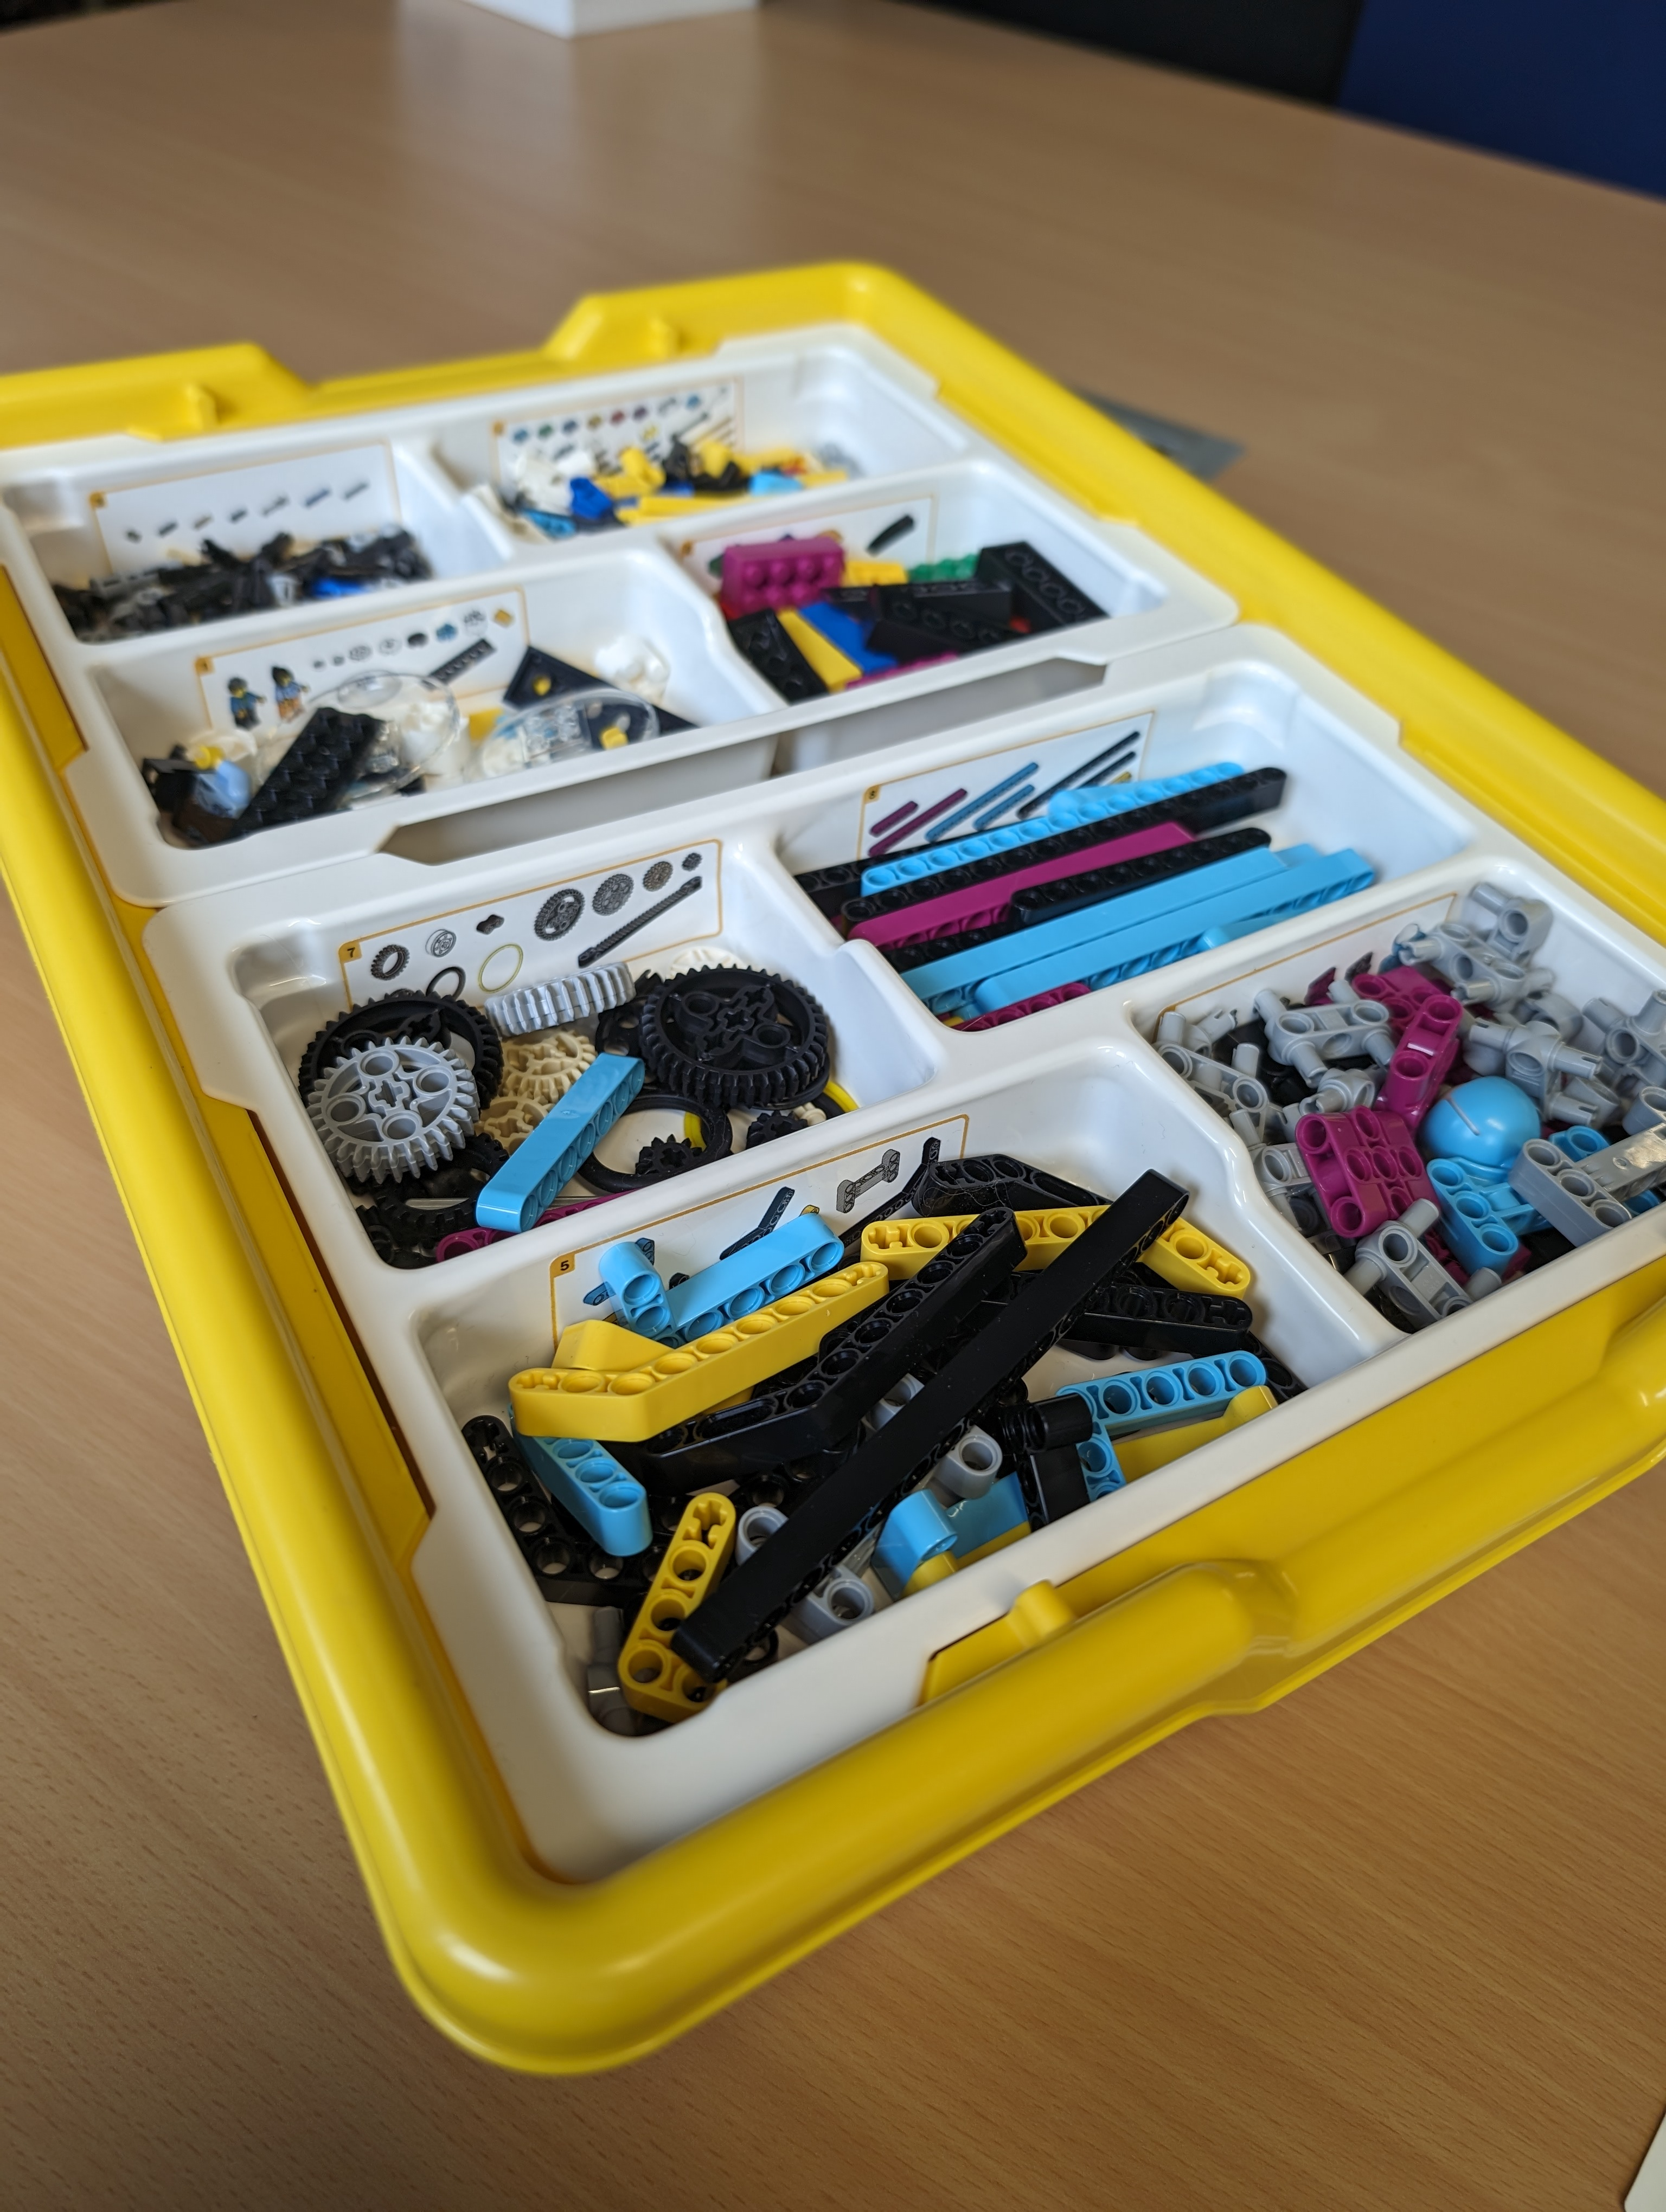
\includegraphics[width=\linewidth]{Figures/lego2.jpg}
\caption{All contents of the LEGO® Education SPIKE™ Prime kit}
\Description{LEGO® bricks, wires and components of the kit}
\label{fig:lego}
\end{figure}

\paragraph{INTIA}

INTIA was a research project that focused on the inclusive development of methods and technologies to help people with disabilities and educational support cope with everyday life. It ran from 2019 to 2023 and included, among other things, a suitcase.

The INTIA suitcase\footnote{\url{https://intia.de/intia-koffer/}~(last accessed: January 21, 2025)\label{intiafootnote}}
is intended to provide initial access to technology and consists of an experience module and a design module. The ''Experience'' module contains an escape game, a technology fan that acts as an encyclopedia, and various components in the form of sensors. The ''Design'' module consists of various sets of cards, an idea cube that encourages creativity, and programming tiles that provide an easy introduction to a programming language. The suitcase and its contents are shown in figure~\ref{ref:intia}.

\begin{figure}[h!]
\centering
\begin{minipage}{0.45\linewidth}
\centering
\includegraphics[width=\linewidth]{Figures/INTIA Koffer Escape Game.jpg}
\end{minipage}
\begin{minipage}{0.45\linewidth}
\centering
\includegraphics[width=\linewidth]{Figures/INTIA Koffer 4.jpg}
\end{minipage}
\caption{INTIA suitcase and contents\footref{intiafootnote}}
\label{ref:intia}
\Description{Different wires, a tablet and technical building blocks laying on a table. A black suitcase filled with colorful cards, dices and tiles.}
\end{figure}
\paragraph{MOXD IoT Kit}

The MoxdLab at Cologne University of Applied Sciences has developed an IoT kit\footnote{\url{https://moxd.io/iotkit}~(last accessed: January 21, 2025)} that can primarily be used for prototyping. Among other things, it is used in the introductory module ''Introduction to Media Informatics'' and is intended to serve as a first introduction to programming. The kit can be used completely without code, but still offers the possibility to do so.

The IoT kit contains a Raspberry Pie in combination with a Groveshield, the Groveshield connectors, and various sensors and actuators, as shown in figure~\ref{fig:iot-kit}. It also includes a cheatsheet that lists a description of the nodes and useful combinations of nodes for various use cases. A Node RED instance runs on the Raspberry Pie, which can be used to work with the components of the kit.

\begin{figure}[h]
\centering
\includegraphics[width=\linewidth]{Figures/iot-kit_emi.jpeg}
\caption{All contents of the IoT Kit}
\Description{Different sensors and actuators, and a Raspberry Pie lying in front of a black suitcase on a wooden table.}
\label{fig:iot-kit}
\end{figure}
\end{comment}

\section{Workshop Konzepte}

Um die unterschiedlichen Altersgruppen und Vorerfahrungen der Schülerinnen und Schüler adäquat abzuholen, wurden im Projekt spezifische Workshop-Konzepte entwickelt. Diese folgen einer gemeinsamen didaktischen Grundstruktur, variieren jedoch stark in Inhalt, Komplexität und methodischem Ansatz.

\subsection*{Allgemeine Agenda und Struktur}

Unabhängig von der Zielgruppe folgt jeder Workshop einem bewährten strukturellen Rahmen, der eine Balance aus Input, Aktivität und Reflexion gewährleistet:

\begin{itemize}
    \item \textbf{Einführung und Zielsetzung:} Klare Transparenz schaffen -- Was machen wir heute? Wozu dient das Endprodukt?
    \item \textbf{Theoretische Grundlagen:} Kurze, prägnante Vermittlung der notwendigen Konzepte (z. B. ``Was ist eine Schleife?''), oft unterstützt durch ``Unplugged''-Methoden.
    \item \textbf{Praktische Übungen:} Der Kern des Workshops. Hier wird entwickelt, gebaut und programmiert.
    \item \textbf{Feedback und Diskussion:} Vorstellung der Ergebnisse (Show \& Tell) und Reflexion über aufgetretene Probleme (Debugging-Kultur).
    \item \textbf{Abschluss und Zusammenfassung:} Sicherung der Lernergebnisse.
    \item \textbf{Gimmick:} Jeder Workshop endet mit einem besonderen Highlight oder einem ``Take-Home''-Element (z. B. das Spiel auf dem eigenen Handy, ein physisches Artefakt), um eine positive emotionale Verankerung zu sichern.
\end{itemize}

\subsection*{Zielgruppenspezifische Ausrichtung}

Damit die Workshops erfolgreich sind, basieren sie auf drei zentralen Säulen, die für alle Altersstufen gelten:

\begin{enumerate}
    \item \textbf{Interaktion:} Frontalunterricht wird auf ein Minimum reduziert. Der Fokus liegt auf dem ``Machen''.
    \item \textbf{Relevanz:} Die Inhalte müssen an die Lebenswelt der Teilnehmenden anknüpfen (z. B. Smartphone-Apps, Spiele).
    \item \textbf{Gruppenarbeit:} Die Förderung von Teamkompetenzen durch kooperative Arbeitsformen (Pair Programming, Projektteams).
\end{enumerate}

\subsection*{Altersdifferenzierte Konzepte}

Die inhaltliche Ausgestaltung orientiert sich an der kognitiven Entwicklung und den typischen Interessen der jeweiligen Altersstufen:

\subsubsection{Altersgruppe 13–15 Jahre (Klasse 7–9): Der spielerische Einstieg}

In dieser Phase steht der niedrigschwellige Zugang im Vordergrund. Vorerfahrungen werden nicht vorausgesetzt, aber aktiv abgefragt, um Gruppen homogen zu bilden.

\begin{itemize}
    \item \textbf{Inhalte:} Fokus auf visuellen, blockbasierten Sprachen wie \textit{Scratch} oder dem \textit{MIT App Inventor}.
    \item \textbf{Ziel:} Schnelle Sichtbarkeit von Ergebnissen. Das Verständnis von Algorithmen wird spielerisch erlernt, ohne durch Syntax-Fehler frustriert zu werden. Die Erstellung eigener kleiner Apps oder Spiele motiviert durch direkten Alltagsbezug.
\end{itemize}

\subsubsection{Altersgruppe 15–17 Jahre (Klasse 9–11): Der Übergang zur Textprogrammierung}

Hier erfolgt oft der Schritt von der visuellen zur textuellen Programmierung. Die Projekte werden komplexer und technischer.

\begin{itemize}
    \item \textbf{Inhalte:} Einführung in textbasierte Sprachen (z. B. \texttt{C}) oder fortgeschrittenes Game Development.
    \item \textbf{Projektbeispiel:} Die Programmierung eines funktionstüchtigen Taschenrechners oder eines komplexeren Spiels.
    \item \textbf{Fokus:} Vertiefung des algorithmischen Verständnisses, Einführung in Datentypen und logische Operatoren. Die Schülerinnen und Schüler lernen, abstraktere Probleme in Code zu übersetzen.
\end{itemize}

\subsubsection{Altersgruppe 18–19 Jahre (Oberstufe / Berufskolleg): Simulation der Berufswirklichkeit}

Bei den ältesten Teilnehmenden verschiebt sich der Fokus vom reinen \textit{Coden} hin zum professionellen Prozess der Softwareentwicklung.

\begin{itemize}
    \item \textbf{Inhalte:} Durchlaufen eines kompletten Software-Entwicklungs-Zyklus.
    \item \textbf{Methodik:} Simulation eines realen Entwicklungsteams. Die Teilnehmenden übernehmen verschiedene Rollen (z. B. Projektmanagement, Frontend-Entwicklung, Backend-Entwicklung, Testing).
    \item \textbf{Ziel:} Verständnis für die Arbeitsteilung und die Prozesse in der IT-Industrie (Requirements Engineering, agile Methoden) entwickeln, als Vorbereitung auf Studium oder Ausbildung.
\end{itemize}

\chapter{Projekte}

Die im Rahmen von \glqq Coding Culture Oberberg\grqq{} entwickelte Web-App fungiert als zentraler Hub für alle Beteiligten: Sie ist Wissensspeicher, Materialdatenbank und Community-Plattform in einem. Ziel der Anwendung ist es, die Hürden für den Einstieg in den Informatikunterricht so gering wie möglich zu halten, indem alle Ressourcen an einem Ort gebündelt und visuell ansprechend aufbereitet werden.

Dieses Kapitel gibt einen Überblick über den Aufbau der Plattform und stellt beispielhaft drei Projekte vor, die im Rahmen der Initiative entstanden sind und evaluiert wurden.

\section{Aufbau der Web-App}

Die Struktur der App wurde bewusst übersichtlich gehalten, um eine intuitive Navigation zu ermöglichen. Die Hauptbereiche gliedern sich wie folgt:

\begin{description}
    \item[Landing Page] Der Einstiegspunkt bietet prägnante Informationen über das Gesamtprojekt, die beteiligten Partner und die übergeordneten Ziele der Initiative. Sie dient als Visitenkarte und als Orientierungshilfe.
    \item[Projekte] Das Herzstück der Anwendung. Hier finden Lehrkräfte eine gefilterte Übersicht aller evaluierten Coding-Projekte. Jedes Projekt wird übersichtlich mit Schwierigkeitsgrad, benötigter Zeit und den adressierten Lernzielen dargestellt.    
    \item[Didaktik] Dieser Bereich fasst die pädagogischen Erkenntnisse zusammen, die aus den Interviews mit Lehrkräften gewonnen wurden. Er dient als theoretischer Unterbau für die praktische Arbeit im Klassenzimmer.
    \item[Muster (Patterns)] Hier werden didaktische Entwurfsmuster veröffentlicht, die sich im Projektverlauf als \glqq Best Practices\grqq{} herauskristallisiert haben. Sie bieten Lösungen für wiederkehrende pädagogische Herausforderungen im Informatikunterricht.    
    \item[Vorlagen] Ein Download-Bereich für standardisierte Templates. Von Projektkarten über Präsentationsvorlagen bis hin zu Feedbackbögen können Lehrkräfte hier Materialien herunterladen, um den Unterricht effizient vorzubereiten.
\end{description}

\section{Highlights}

Um die theoretischen Konzepte mit Leben zu füllen, werden im Folgenden drei beispielhafte Projekte vorgestellt, die unterschiedliche didaktische Schwerpunkte setzen.

\subsection{Mission Weltraum}

Dieses Projekt entstand aus der konkreten Aufgabenstellung, ein Konzept für einen \glqq Coding-Koffer\grqq{} für die Klassen 5 bis 7 zu entwickeln. Die Herausforderung bestand darin, abstrakte Programmierkonzepte lehrkraftfreundlich, motivierend und binnendifferenziert zu vermitteln, ohne die Schülerinnen und Schüler durch trockene Theorie zu frustrieren.

\subsubsection*{Das Konzept: Storytelling trifft Gamification}
Um die Motivation der Lernenden dauerhaft zu sichern, bettet das Projekt alle Aufgaben in eine durchgehende \textbf{Raumschiff-Geschichte} ein. Die Storyline gibt Struktur und einen Sinnzusammenhang für die fünf Lerneinheiten (Kapitel) à 45 Minuten:

\begin{enumerate}
    \item \textbf{Sequenzen:} Der Start der Mission.
    \item \textbf{Schleifen \& Bedingungen:} Navigation durch Asteroidenfelder.
    \item \textbf{Variablen:} Ressourcenmanagement an Bord.
    \item \textbf{Algorithmen \& Methoden:} Komplexe Flugmanöver.
    \item \textbf{Finale:} Wiederholungs-Quiz und ein Scratch-Abschlussprojekt.
\end{enumerate}

\subsubsection*{Didaktischer Ansatz: Rollenspiel und Skeuomorphismus}
Die Klasse wird in 4er-Gruppen aufgeteilt. Jedes Gruppenmitglied übernimmt pro Lerneinheit die Rolle eines Charakters aus der Geschichte (z.\,B. Navigator, Ingenieur). Diese Rollen rotieren, sodass jedes Kind unterschiedliche Verantwortungen trägt und die Teamdynamik gestärkt wird.

Ein Kernmerkmal ist die Nutzung von \textbf{Abstraktionen und Skeuomorphismus}: Technische Konzepte werden durch physische Gegenstände erklärt. So werden Variablen beispielsweise nicht abstrakt als Speicheradressen definiert, sondern durch echte Becher repräsentiert, in denen Werte \glqq gelagert\grqq{} werden.

\subsubsection*{Der physische Koffer}
Um die Hürde für Lehrkräfte zu minimieren, passt das gesamte Basismaterial in einen einfachen Pappkarton:
\begin{itemize}
    \item Ein USB-Stick mit allen PDFs, digitalen Inhalten und Druckvorlagen.
    \item 8 Becher zur Veranschaulichung des Variablen-Konzepts.
\end{itemize}
Zusätzlich werden lediglich Scheren, Spielfiguren und ein internetfähiges Gerät pro Gruppe benötigt.

\subsection{Das Labyrinth}

Dieses Projekt verbindet handwerkliches Geschick mit algorithmischem Denken und Robotik. Es eignet sich besonders, um den Transfer von Code in die physische Welt zu demonstrieren.

\textbf{Ablauf:}
\begin{enumerate}
    \item \textbf{Bauphase:} Die Schülerinnen und Schüler konstruieren zunächst physisch ein Labyrinth aus Pappe.
    \item \textbf{Programmierung:} Ein Micro:bit-Mikrocontroller, montiert auf einem Maqueen-Roboterchassis, wird programmiert. Ziel ist es, dass der Roboter mithilfe seiner Sensoren (Ultraschall oder Linienfolger) selbstständig Hindernisse erkennt.
    \item \textbf{Algorithmus:} Der Wegfindungs-Algorithmus wird gemeinsam in der Gruppe entwickelt (z.\,B. die \glqq Wandfolger\grqq-Strategie).
    \item \textbf{Wettbewerb:} Den Abschluss bildet ein Rennen: Welcher Roboter bewältigt das Labyrinth am schnellsten?
\end{enumerate}

\subsection{Tug of War}

Basierend auf den \textit{littleBits}-Modulen bietet dieses Projekt einen spielerischen Zugang zu Elektronik und Logik ohne Schreibarbeit am Computer.

\textbf{Konzept:}\\
Schülerinnen und Schüler bauen eine digitale Version des klassischen Tauziehens. Hierbei kommen Eingabemodule (Buttons/Sensoren) und Ausgabemodule (LED-Leisten oder Motoren) zum Einsatz. Durch schnelles Drücken oder Interagieren muss ein Signal auf die eigene Seite \glqq gezogen\grqq{} werden. Das Projekt fördert das Verständnis für digitale Signale, Zustandswechsel und den Aufbau einfacher Schaltkreise.

% TODO: Zusammenhang + Checklist Generator

\chapter{Beitrag}

Das Projekt \glqq Coding Culture Oberberg\grqq{} ist kein statisches Werk, sondern eine lebendige Plattform, die von den Erfahrungen und Ideen der Community lebt. Die Web-App und die Materialsammlung sind als Open-Source-Projekt konzipiert. Das bedeutet: Jede Lehrkraft, jede Schülerin und jeder Schüler sowie Entwicklerinnen und Entwickler sind eingeladen, Fehler zu korrigieren, neue Features zu entwickeln oder eigene Projektideen beizusteuern.

Dieses Kapitel beschreibt, wie Sie technisch zur Web-App beitragen, wie Sie neue Projekte in das System einspeisen und wie Sie die bereitgestellten Vorlagen nutzen und erweitern können.

\section{Anleitung zur Weiterentwicklung der Web App}

Die Web App ist das Herzstück des Projekts. Sie dient als Katalog für Projekte, als Wissensspeicher und als Werkzeugkasten für den Unterricht. Gehostet wird die Anwendung über \textbf{GitHub Pages}, der Quellcode liegt offen auf dem dazugehörigen GitHub-Repository.
% TODO: Links einfügen

\subsection*{Der Technologie-Stack}
Für technisch interessierte Mitstreiter: Die App basiert auf einem modernen, performanten Stack:
\begin{itemize}
    \item \textbf{Svelte:} Als Frontend-Framework für eine reaktive und schnelle Benutzeroberfläche.
    \item \textbf{shadcn/ui:} Für ein zugängliches, konsistentes und ansprechendes Design der Komponenten.
\end{itemize}

\subsection*{Zusammenarbeit via GitHub}
Die Kollaboration findet zentral auf der Plattform GitHub statt. Hier gibt es verschiedene Wege, sich einzubringen:

\begin{enumerate}
    \item \textbf{Issues (Fehler melden \& Ideen einbringen):} Wenn Sie einen Fehler (Bug) in der App finden oder eine Idee für eine neue Funktion haben, können Sie im Reiter \textit{Issues} ein neues Ticket erstellen. Beschreiben Sie das Problem so genau wie möglich.
    \item \textbf{Discussions (Austausch):} Über den Tab \textit{Discussions} können Sie in Kontakt mit anderen Lehrkräften und den Entwicklern treten. Hier ist der Platz für pädagogische Fragen, Erfahrungsaustausch oder Diskussionen über Best Practices im Informatikunterricht.
    \item \textbf{Pull Requests (Code beisteuern):} Wer selbst programmieren kann, darf den Code direkt erweitern.
    \begin{itemize}
        \item \textbf{Forken} Sie das Repository (erstellen Sie Ihre eigene Kopie).
        \item Erstellen Sie einen neuen \textbf{Branch} für Ihre Änderung.
        \item Reichen Sie Ihre Änderungen als \textbf{Pull Request (PR)} ein. Das Kern-Team prüft den Code und übernimmt ihn in die Hauptversion.
    \end{itemize}
\end{enumerate}

\subsection*{Git \& GitHub in aller Kürze}
Für Einsteiger in die Versionierung mit Git sind dies die wichtigsten Schritte im Terminal:

\begin{lstlisting}[style=bash]
git clone [URL] 
# Laedt das Repository auf Ihren Rechner.

git checkout -b feature/mein-feature 
# Erstellt einen neuen Arbeitszweig.

git add . 
git commit -m "Beschreibung" 
# Speichert Ihre Aenderungen.

git push origin feature/mein-feature 
# Laedt die Aenderungen hoch, um einen Pull Request zu stellen.
\end{lstlisting}

\section{Entwicklung und Integration neuer Projekte}

Damit die Plattform wächst, brauchen wir stetig neue Projektideen. Das Hinzufügen eines neuen Projekts in die Web-App erfordert \textbf{keine Programmierkenntnisse} in Svelte. Die App generiert die Projektübersicht dynamisch aus einer zentralen Datendatei.

\subsection*{Der Prozess über das GitHub-Interface}
Sie können neue Projekte direkt im Browser über die GitHub-Oberfläche hinzufügen:

\begin{enumerate}
    \item Navigieren Sie im Repository zur Datei \texttt{app/static/data/projects/template.json} (oder dem entsprechenden Daten-Ordner).
    \item Klicken Sie auf das Stift-Symbol (\textit{Edit this file}).
    \item Fügen Sie einen neuen Eintrag nach dem untenstehenden JSON-Schema hinzu.
    \item Klicken Sie unten auf \textit{Commit changes} und wählen Sie \textit{Create a new branch for this commit and start a pull request}. Damit schlagen Sie Ihr neues Projekt zur Aufnahme vor.
\end{enumerate}

\subsection*{Die JSON-Struktur}
Ein Projekt wird durch ein JSON-Objekt definiert. Hier ist die Vorlage mit Erklärungen zu den einzelnen Feldern:

\begin{lstlisting}[language=json]
{
	"id": "UUID",
	"name": "Name",
	"description": "Beschreibung",
	"product": "Produkt",
	"content": [
		"Keyword 1",
		"Keyword 2",
		"Keword 3"
	],
	"complexity": 1,
	"language": ["Python"],
	"minDuration": 30,
	"maxDuration": 60,
	"minGroup": 1,
	"maxGroup": 3,
	"type": "Konsolenspiel",
	"materials": [
		"Computer",
		"Schere",
		"Papier"
	]
}
\end{lstlisting}

\subsection*{Erklärung der Felder}
\begin{description}
    \item[id] Eine einzigartige Identifikationsnummer. Nutzen Sie einen Online-UUID-Generator, um eine zufällige ID zu erzeugen. Dies verhindert Datenbankkonflikte.
    \item[name \& description] Titel und Teaser-Text, der auf der Übersichtskarte in der App erscheint.
    \item[product] Das zentrale Produkt, um das es sich dreht.
    \item[content] Eine Liste von Lerninhalten (Tags), nach denen Nutzer filtern können.
    \item[complexity] Eine Skala von 1 (Einfach) bis 3 (Schwer).
    \item[language] Die verwendete(n) Programmiersprache(n).
    \item[duration] Zeitrahmen in Minuten (von/bis).
    \item[group] Gruppengröße (von/bis).
    \item[type] Die Art von Projekt, z.B. Einplatinencomputer, Brettspiel, etc. 
    \item[materials] Physische oder digitale Materialien, die vorbereitet werden müssen.
\end{description}

Sobald Ihr Pull Request akzeptiert ist, erscheint das Projekt automatisch in der Web-App und kann von Lehrkräften überall genutzt werden.

\section{Nutzung und Anpassung von Vorlagen}

Um den Vorbereitungsaufwand für Lehrkräfte zu minimieren, bietet die Web-App einen eigenen Reiter \textbf{\glqq Vorlagen\grqq{}}. Hier finden sich standardisierte Dokumente, die für einen reibungslosen Ablauf der Projekte sorgen. Diese Vorlagen sind ebenfalls Open Source und können bei Bedarf angepasst werden.

Folgende Kategorien stehen zum Download bereit:

\subsection{Projektkarten}
Dies sind visuell aufbereitete Kurzübersichten (\textit{One-Pagers}) für jedes Projekt. Sie eignen sich hervorragend für offene Lernphasen oder Stationenlernen. Schülerinnen und Schüler können anhand der Karten selbstständig entscheiden, welches Projekt sie bearbeiten möchten. Sie enthalten den Titel, das Zielprodukt, den Schwierigkeitsgrad und die benötigte Zeit auf einen Blick.

\subsection{Präsentationsvorlagen}
Die bereitgestellten Folien-Templates geben eine Struktur vor, um den Unterricht, orientiert an den Projekten und im Workshop-Charakter, zu präsentieren.

\subsection{Feedbackbögen zur Evaluation}
Um die Qualität des Unterrichts und der Materialien zu sichern, stehen Feedbackbögen bereit. Diese können von den Lernenden ausgefüllt werden, um Rückmeldung zu den Projekten zu geben.

\subsection{Anleitungstemplates (Handreichungen)}
Für jedes neue Projekt können zusätzlich Schülerhandreichungen erstellt werden. Das Anleitungstemplate bietet eine didaktisch sinnvolle Struktur und ein einheitliches Design.
\\

Wir ermutigen alle Nutzenden, verbesserte Versionen dieser Vorlagen oder gänzlich neue Hilfsmittel über den oben beschriebenen GitHub-Workflow wieder in das Projekt zurückfließen zu lassen.

\end{document}
